% Options for packages loaded elsewhere
\PassOptionsToPackage{unicode}{hyperref}
\PassOptionsToPackage{hyphens}{url}
%
\documentclass[
]{article}
\usepackage{amsmath,amssymb}
\usepackage{lmodern}
\usepackage{iftex}
\ifPDFTeX
  \usepackage[T1]{fontenc}
  \usepackage[utf8]{inputenc}
  \usepackage{textcomp} % provide euro and other symbols
\else % if luatex or xetex
  \usepackage{unicode-math}
  \defaultfontfeatures{Scale=MatchLowercase}
  \defaultfontfeatures[\rmfamily]{Ligatures=TeX,Scale=1}
\fi
% Use upquote if available, for straight quotes in verbatim environments
\IfFileExists{upquote.sty}{\usepackage{upquote}}{}
\IfFileExists{microtype.sty}{% use microtype if available
  \usepackage[]{microtype}
  \UseMicrotypeSet[protrusion]{basicmath} % disable protrusion for tt fonts
}{}
\makeatletter
\@ifundefined{KOMAClassName}{% if non-KOMA class
  \IfFileExists{parskip.sty}{%
    \usepackage{parskip}
  }{% else
    \setlength{\parindent}{0pt}
    \setlength{\parskip}{6pt plus 2pt minus 1pt}}
}{% if KOMA class
  \KOMAoptions{parskip=half}}
\makeatother
\usepackage{xcolor}
\IfFileExists{xurl.sty}{\usepackage{xurl}}{} % add URL line breaks if available
\IfFileExists{bookmark.sty}{\usepackage{bookmark}}{\usepackage{hyperref}}
\hypersetup{
  hidelinks,
  pdfcreator={LaTeX via pandoc}}
\urlstyle{same} % disable monospaced font for URLs
\usepackage[margin=1in]{geometry}
\usepackage{color}
\usepackage{fancyvrb}
\newcommand{\VerbBar}{|}
\newcommand{\VERB}{\Verb[commandchars=\\\{\}]}
\DefineVerbatimEnvironment{Highlighting}{Verbatim}{commandchars=\\\{\}}
% Add ',fontsize=\small' for more characters per line
\usepackage{framed}
\definecolor{shadecolor}{RGB}{248,248,248}
\newenvironment{Shaded}{\begin{snugshade}}{\end{snugshade}}
\newcommand{\AlertTok}[1]{\textcolor[rgb]{0.94,0.16,0.16}{#1}}
\newcommand{\AnnotationTok}[1]{\textcolor[rgb]{0.56,0.35,0.01}{\textbf{\textit{#1}}}}
\newcommand{\AttributeTok}[1]{\textcolor[rgb]{0.77,0.63,0.00}{#1}}
\newcommand{\BaseNTok}[1]{\textcolor[rgb]{0.00,0.00,0.81}{#1}}
\newcommand{\BuiltInTok}[1]{#1}
\newcommand{\CharTok}[1]{\textcolor[rgb]{0.31,0.60,0.02}{#1}}
\newcommand{\CommentTok}[1]{\textcolor[rgb]{0.56,0.35,0.01}{\textit{#1}}}
\newcommand{\CommentVarTok}[1]{\textcolor[rgb]{0.56,0.35,0.01}{\textbf{\textit{#1}}}}
\newcommand{\ConstantTok}[1]{\textcolor[rgb]{0.00,0.00,0.00}{#1}}
\newcommand{\ControlFlowTok}[1]{\textcolor[rgb]{0.13,0.29,0.53}{\textbf{#1}}}
\newcommand{\DataTypeTok}[1]{\textcolor[rgb]{0.13,0.29,0.53}{#1}}
\newcommand{\DecValTok}[1]{\textcolor[rgb]{0.00,0.00,0.81}{#1}}
\newcommand{\DocumentationTok}[1]{\textcolor[rgb]{0.56,0.35,0.01}{\textbf{\textit{#1}}}}
\newcommand{\ErrorTok}[1]{\textcolor[rgb]{0.64,0.00,0.00}{\textbf{#1}}}
\newcommand{\ExtensionTok}[1]{#1}
\newcommand{\FloatTok}[1]{\textcolor[rgb]{0.00,0.00,0.81}{#1}}
\newcommand{\FunctionTok}[1]{\textcolor[rgb]{0.00,0.00,0.00}{#1}}
\newcommand{\ImportTok}[1]{#1}
\newcommand{\InformationTok}[1]{\textcolor[rgb]{0.56,0.35,0.01}{\textbf{\textit{#1}}}}
\newcommand{\KeywordTok}[1]{\textcolor[rgb]{0.13,0.29,0.53}{\textbf{#1}}}
\newcommand{\NormalTok}[1]{#1}
\newcommand{\OperatorTok}[1]{\textcolor[rgb]{0.81,0.36,0.00}{\textbf{#1}}}
\newcommand{\OtherTok}[1]{\textcolor[rgb]{0.56,0.35,0.01}{#1}}
\newcommand{\PreprocessorTok}[1]{\textcolor[rgb]{0.56,0.35,0.01}{\textit{#1}}}
\newcommand{\RegionMarkerTok}[1]{#1}
\newcommand{\SpecialCharTok}[1]{\textcolor[rgb]{0.00,0.00,0.00}{#1}}
\newcommand{\SpecialStringTok}[1]{\textcolor[rgb]{0.31,0.60,0.02}{#1}}
\newcommand{\StringTok}[1]{\textcolor[rgb]{0.31,0.60,0.02}{#1}}
\newcommand{\VariableTok}[1]{\textcolor[rgb]{0.00,0.00,0.00}{#1}}
\newcommand{\VerbatimStringTok}[1]{\textcolor[rgb]{0.31,0.60,0.02}{#1}}
\newcommand{\WarningTok}[1]{\textcolor[rgb]{0.56,0.35,0.01}{\textbf{\textit{#1}}}}
\usepackage{longtable,booktabs,array}
\usepackage{calc} % for calculating minipage widths
% Correct order of tables after \paragraph or \subparagraph
\usepackage{etoolbox}
\makeatletter
\patchcmd\longtable{\par}{\if@noskipsec\mbox{}\fi\par}{}{}
\makeatother
% Allow footnotes in longtable head/foot
\IfFileExists{footnotehyper.sty}{\usepackage{footnotehyper}}{\usepackage{footnote}}
\makesavenoteenv{longtable}
\usepackage{graphicx}
\makeatletter
\def\maxwidth{\ifdim\Gin@nat@width>\linewidth\linewidth\else\Gin@nat@width\fi}
\def\maxheight{\ifdim\Gin@nat@height>\textheight\textheight\else\Gin@nat@height\fi}
\makeatother
% Scale images if necessary, so that they will not overflow the page
% margins by default, and it is still possible to overwrite the defaults
% using explicit options in \includegraphics[width, height, ...]{}
\setkeys{Gin}{width=\maxwidth,height=\maxheight,keepaspectratio}
% Set default figure placement to htbp
\makeatletter
\def\fps@figure{htbp}
\makeatother
\setlength{\emergencystretch}{3em} % prevent overfull lines
\providecommand{\tightlist}{%
  \setlength{\itemsep}{0pt}\setlength{\parskip}{0pt}}
\setcounter{secnumdepth}{-\maxdimen} % remove section numbering
\ifLuaTeX
  \usepackage{selnolig}  % disable illegal ligatures
\fi

\author{}
\date{\vspace{-2.5em}}

\begin{document}

\hypertarget{new-estimations-of-delta-r-values-for-the-south-eastern-pacific-obtained-from-marine20}{%
\section{New estimations of delta R values for the South-eastern Pacific
obtained from
Marine20}\label{new-estimations-of-delta-r-values-for-the-south-eastern-pacific-obtained-from-marine20}}

\hypertarget{contents}{%
\subsection{Contents}\label{contents}}

\begin{itemize}
\tightlist
\item
  \protect\hyperlink{abstract}{Abstract}
\item
  \protect\hyperlink{introduction}{Introduction}
\item
  \protect\hyperlink{materials-and-methods}{Materials and methods}
\item
  \protect\hyperlink{principal-outcomes}{Principal outcomes}
\item
  \protect\hyperlink{ux5cux23discussion}{Discussion}
\item
  \protect\hyperlink{conclusions}{Conclusions}
\item
  \protect\hyperlink{references}{References}
\item
  \protect\hyperlink{r-code}{R code}
\end{itemize}

\hypertarget{abstract}{%
\subsection{Abstract}\label{abstract}}

Radiocarbon (C-14) is a cosmogenic radionuclide produced in the upper
atmosphere that is frequently used in paleoceanography to date sediments
cores. However, dating marine sediment records have an important
particularity, given that contemporaneous terrestrial and marine
organism have different 14-C ages because the ocean is a source of C-14
and thus marine organisms appear to be older than contemporaneous
terrestrial organisms.

This effect is called marine reservoir effect (MRE), it varies in space
and time as a function of changes in upwelling intensity and the origin
of the upwelled waters, and thus needs to be considered while dating
marine sediment cores. Recently an internationally agreed marine
radiocarbon age calibration curve (Marine20) was released and provides a
global average marine record of radiocarbon from 0 to 55 calibrated
Kiloyears before to present, thus serving as a baseline for regional
oceanic variation.

Here we compare the marine reservoir ages (MRA) obtained from the
previous version with the new calibration curve based on 86 published,
marine-terrestrial pairs samples obtained in the Eastern Pacific Ocean
between 0 to 50°S. We applied a bootstrapping method and the output data
were sorted for spatial position and time period. Then, we calculated
the MRA by error propagation and generalized additive model. According
to our results, the MRA show a pattern of time-space distribution at
millennial time scales, with larger MRA ages north of 22°S . These
observations suggest that oceanic circulation is a key factor that
modulated MRA during last 12 Kyr in the Eastern Tropical South Pacific.

Moreover, the estimated MRA using the new radiocarbon age calibration
curve is up to \textasciitilde400 years higher compared to the MRA
obtained using the previous calibration curve, indicating that the
timing of paleoceanographic events based on marine sediment records need
to be revised.

\hypertarget{introduction}{%
\subsection{Introduction}\label{introduction}}

Radiocarbon (c-14) has produced by nuclear reaction due to cosmic rays
in the upper atmosphere \textasciitilde15km. Then C-14 is reacted with
molecular oxygen to generate heavy carbon dioxide that is assimilated by
primary producers via photosynthesis, reaching higher trophic levels via
the food chain (Alves et al.,2018).

The distribution of \(\Delta\)\^{}14 C (\^{}14 C/C)

p1: 14C sign on global ocean p2: Water mass 14C in Peru and chile p3:
Citation marine20 curve brief description p4: to update MRA 2011 of (
ortlieb and carre) p5: to show that hipotesis I would test with it

On Earth, there are three carbon isotope 12 (\%), 13(\%) and 14 (\%)
which involved a dynamic and complex process as called Carbon cycle.

This process has signed in atmosphere, ocean and rocks.

In the atmosphere, Nitrogen 14 has transformed to isotope 14 carbon in
10 km.

When researchers are trying of using radiocarbon ages for calendrical
time scale interpretations or comparisons with dates obtained by other
methods would be problematic (Alves et al.~2018).

It is well-known as specific biogeochemistry conditions regional effect
on carbon 14 isotope. It is important to estimate this effect for dating
tools that estimate to radiocarbon age during the last 50 Kyr in several
areas of research. In this work, I update values of marine radiocarbon
age (MRA) according to the calibrated curve (Marine20 \& Shcal20). Also,
I focus on the MRA relationship with space-time variables (latitude,
longitude, calibrated age, and uncertainty age).

\hypertarget{materials-and-methods}{%
\subsection{Materials and methods}\label{materials-and-methods}}

This work estimates the local radiocarbon reservoir effect off
(\(\Delta\)R) Peru to Chile (0 to 50 °S) during the last 12 Kyr BP.
Therefore, I compiled several previous estimations. It was 185 pairs
(Marine and terrestrial samples of different organic materials (wood,
shell and others organic remains). Bellow, I attached the input data
set.

\begin{figure}
\centering
\includegraphics{https://github.com/jasb3110/Radiocarbon-reservoir/blob/db842ff0620d55ea5ca5ceec0d96a369406b6e3c/r.input\%20data1.png?raw=true}
\caption{alt text}
\end{figure}

\begin{figure}
\centering
\includegraphics{https://github.com/jasb3110/Radiocarbon-reservoir/blob/2aa2f1dd8cfb7737d761e79f91086531b959a368/r.input\%20data2.png?raw=true}
\caption{alt text}
\end{figure}

I used a Bchron package in R to estimate the maximum probability of
calibrated marine and terrestrial age according to Marine20 and Shcal20,
respectively. Then I calculated the difference between each pair under
bootstrapping suggested by Russell et al.~2011. After that, I reduced
the pool data from 185 to 90 samples for decreasing the overweight of
repeated data. So that, I solve this issue, using error weight means
deleting extra values and reducing error calibration.

I sorted of data (without repeated data) for period time: Early Holocene
(EH) was 11.5 to 7 Kyr BP, Mid Holocene (MH) was 7 to 4 Kyr BP, Late
Holocene (LH) was 4 to 0.2 Kyr BP, and Current warming period (CWP) is
last 200 years; space variables: latitude and longitude; calibrated age:
maximum probability age and Uncertainty of maximum probability age;
\(\Delta\) R: estimated value and its uncertainty.

Next, I did do a Factorial multivariate analysis, using the Factominer
package, and a Generalized analysis model(GAM), using mgcv package, of
86 pairs of data. Finally, I recalculated MRA according to latitude and
calibrated age before to present (Cal yr BP) in boxes, using the error
weight mean for decreased error propagation.

\hypertarget{principal-outcomes}{%
\subsection{Principal outcomes}\label{principal-outcomes}}

In this part, I would show highlight the results of this
work.Multivariate analysis was based on seven selected variables over
the length of whole data set (n=90). PCA results indicate that most
variance of the data set ∼52\% was encompassed by the first and second
principal components
\protect\hyperlink{principal-component-analysis-ux28pcaux29}{(fig.~1)}.

\hypertarget{principal-component-analysis-pca}{%
\subsubsection{Principal component analysis
(PCA)}\label{principal-component-analysis-pca}}

\begin{longtable}[]{@{}
  >{\centering\arraybackslash}p{(\columnwidth - 0\tabcolsep) * \real{1.0000}}@{}}
\toprule
\begin{minipage}[b]{\linewidth}\centering
\href{https://github.com/jasb3110/Radiocarbon-reservoir/blob/db842ff0620d55ea5ca5ceec0d96a369406b6e3c/AMV.biplot.png?raw=true}{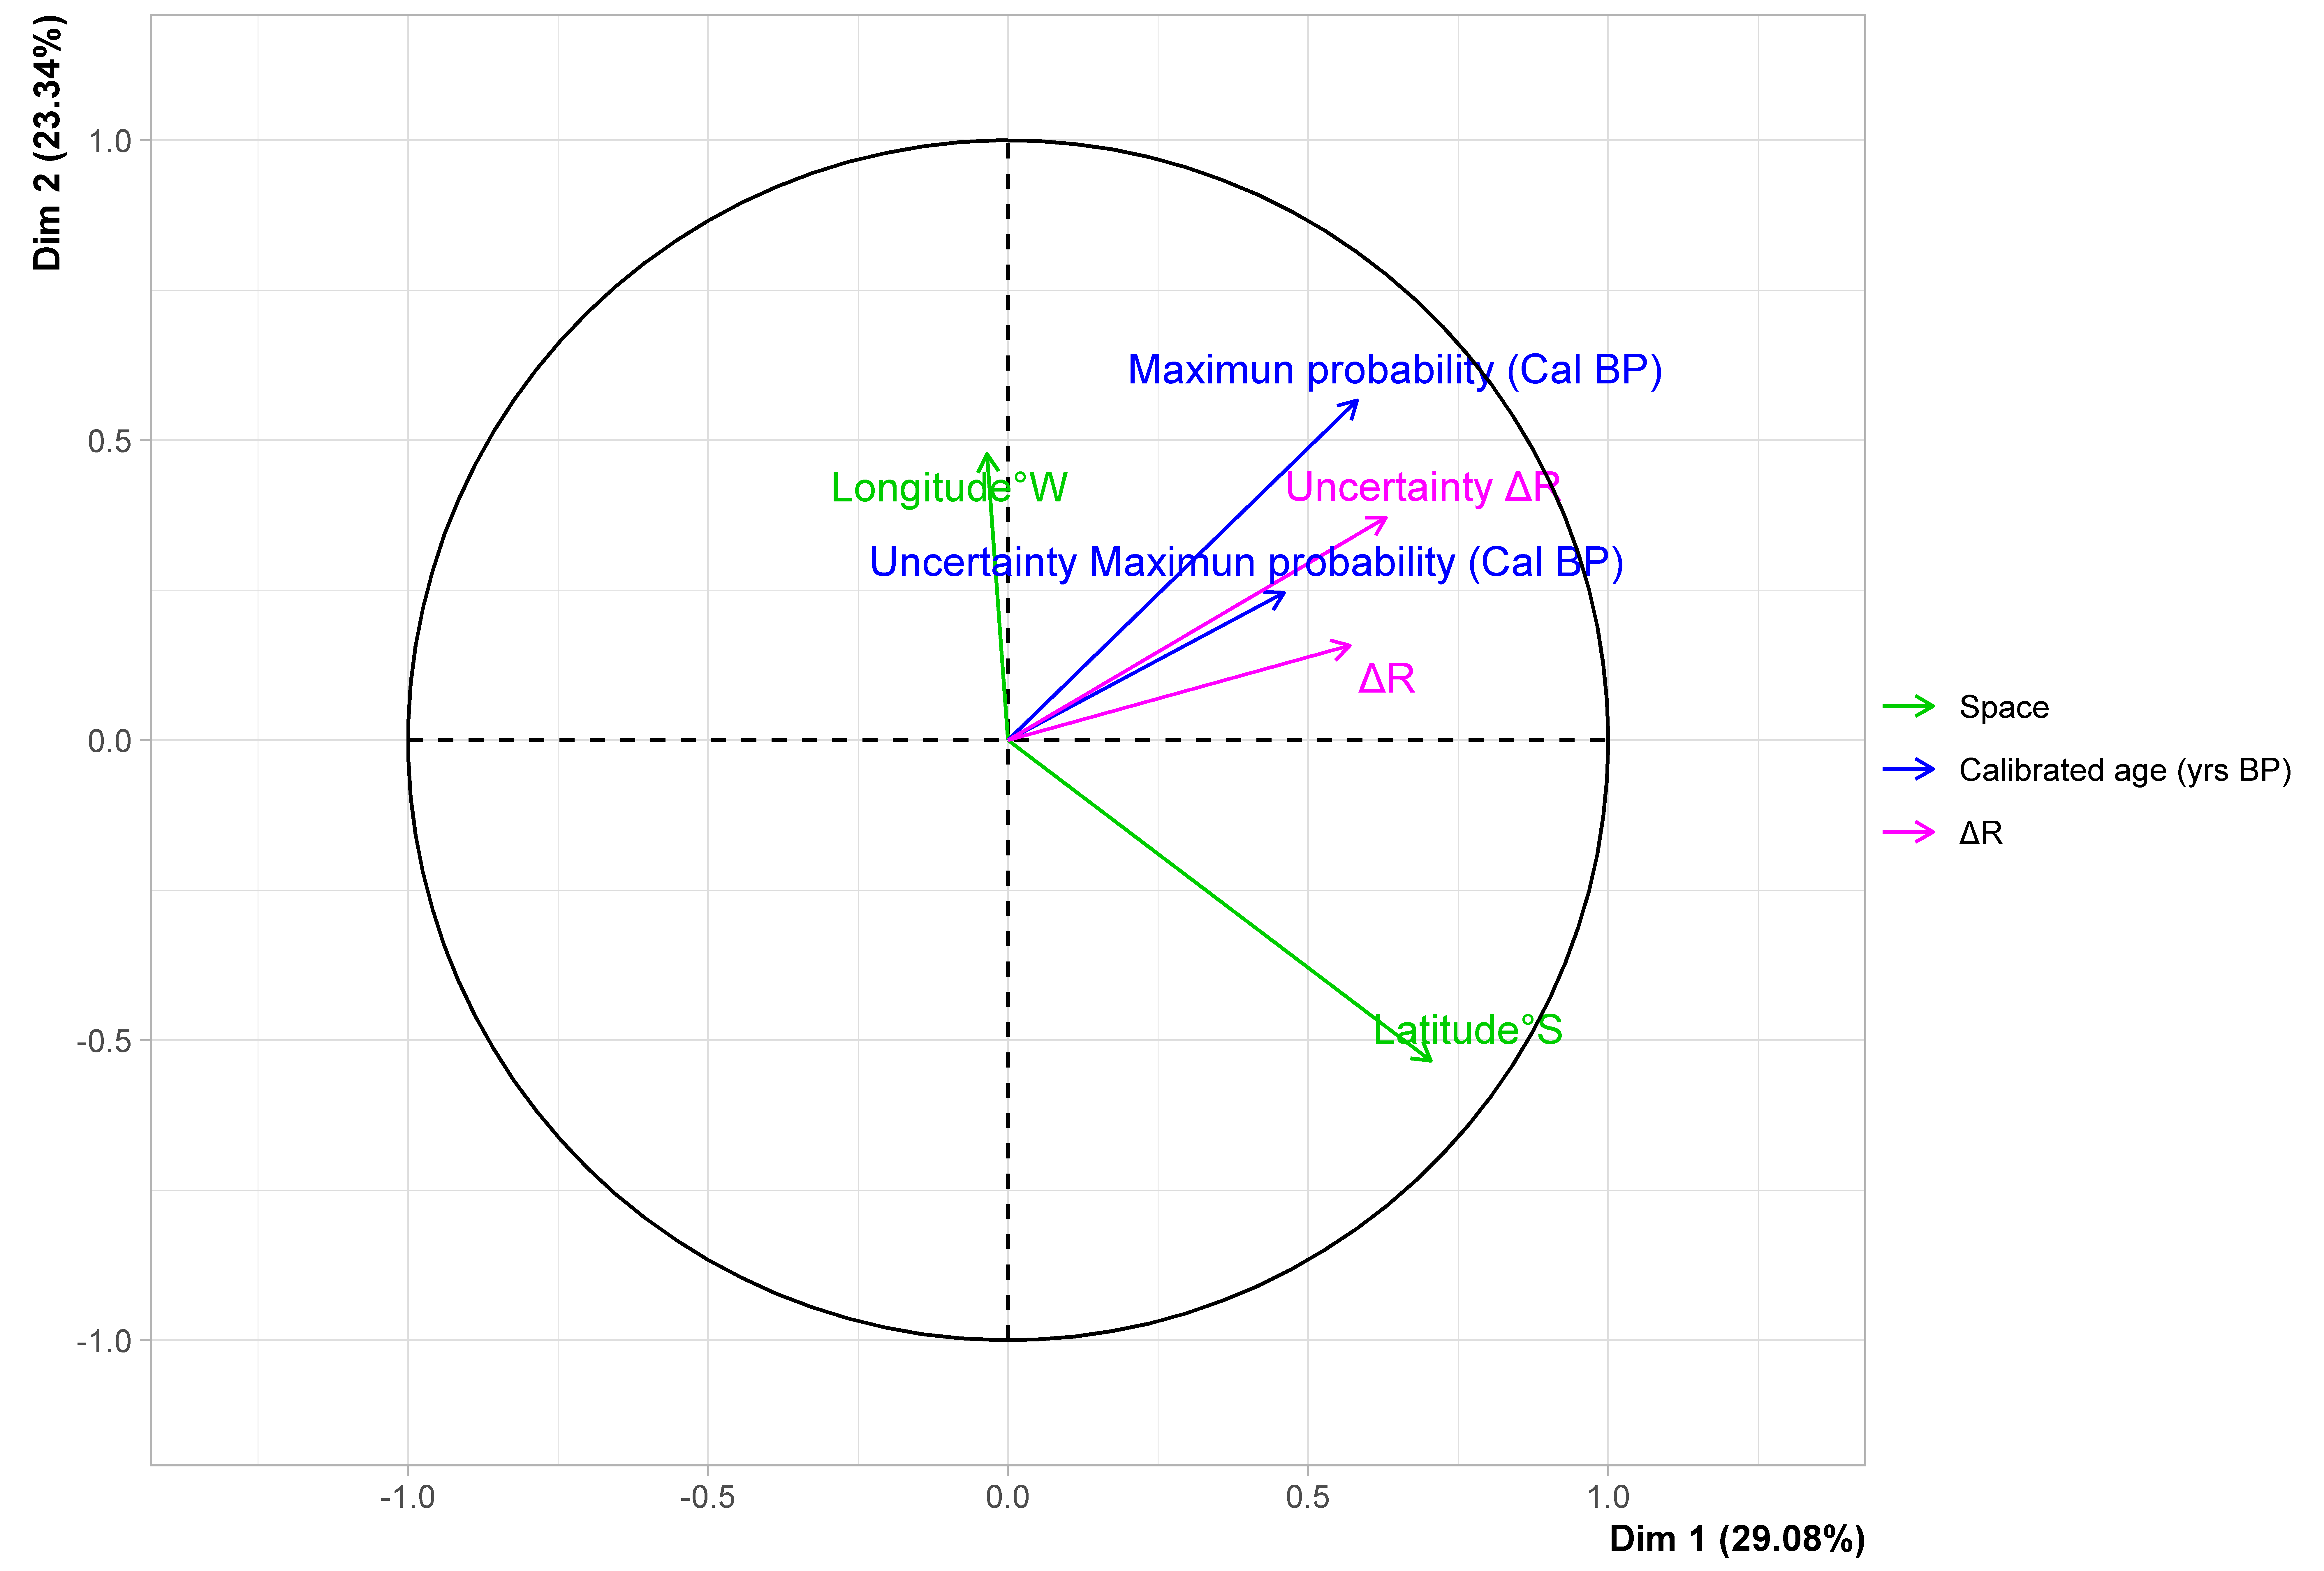
\includegraphics{AMV.biplot.png}}
\end{minipage} \\
\midrule
\endhead
\emph{Figure 1. Biplot of Principal component of data (n=90)} \\
\bottomrule
\end{longtable}

PC1 (∼29\%) is interpreted as signal of latitudinal position. PC1 has
the highest loading for latitude, uncertainty of \(\Delta\) R and
calibrated age. PC2 (∼23\%) is interpreted as signal of longitudinal
position. PC2 has the highest loading for calibrated age, longitude and
uncertainty of \(\Delta\) R
\protect\hyperlink{principal-component-analysis-ux28pcaux29}{(fig.~1)}.

\hypertarget{clusters-of-mra-for-period-time}{%
\subsubsection{Clusters of MRA for period
time}\label{clusters-of-mra-for-period-time}}

\begin{longtable}[]{@{}
  >{\centering\arraybackslash}p{(\columnwidth - 0\tabcolsep) * \real{1.0000}}@{}}
\toprule
\begin{minipage}[b]{\linewidth}\centering
\href{https://github.com/jasb3110/Radiocarbon-reservoir/blob/db842ff0620d55ea5ca5ceec0d96a369406b6e3c/plotellipses.period.png?raw=true}{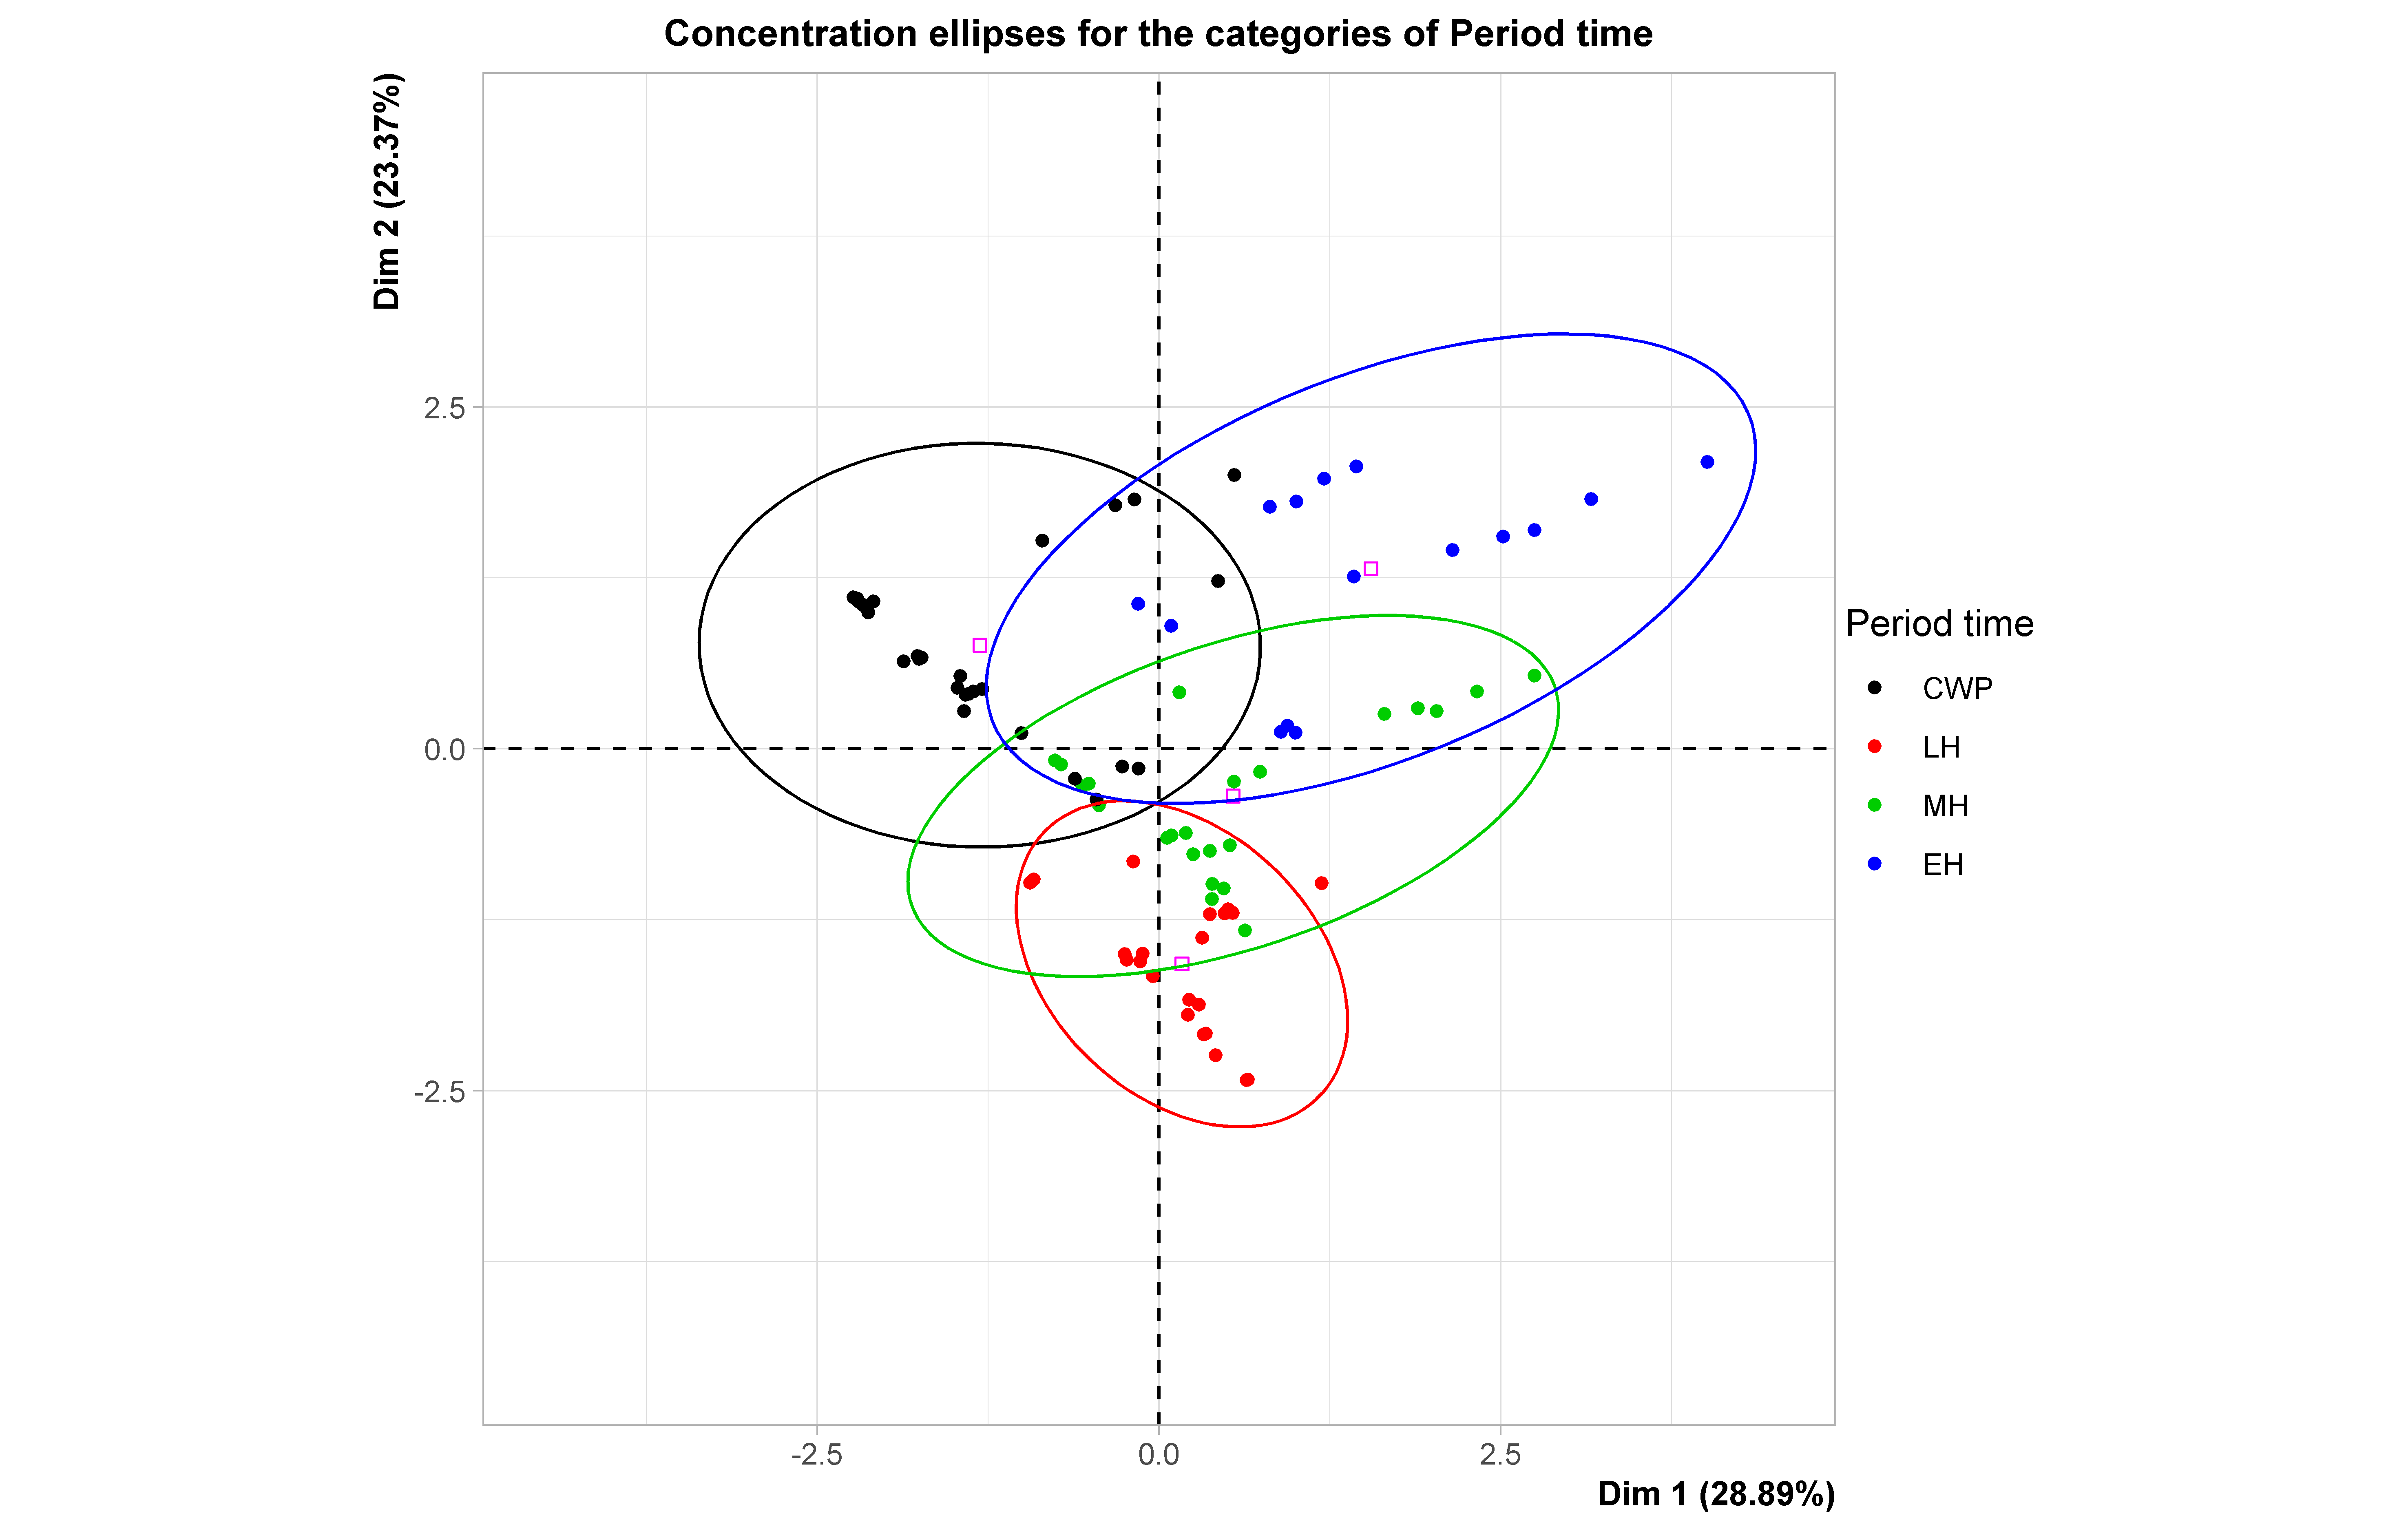
\includegraphics{plotellipses.period.png}}
\end{minipage} \\
\midrule
\endhead
\emph{Figure 2. Concentration ellipses for the categories of period
time. CWP:Current warming period (black), LH:Late Holocene (red), MH:Mid
Holocene (green), EH:Early Holocene (blue)} \\
\bottomrule
\end{longtable}

According to periods, It could be no evidence of a temporal effect on
the MRA during the Holocene except for CWP. Therefore, I noticed a small
difference between the
periods.\protect\hyperlink{Clusters-of-mra-for-period-time}{(fig.2)}.

\hypertarget{latitudinal-distribution-of-mra}{%
\subsubsection{Latitudinal distribution of
MRA}\label{latitudinal-distribution-of-mra}}

Some past works showed the difference in latitudinal of MRA off Peru \&
Chile. However, it did not validate a criterion for dividing in zones
before estimating MRA.

\begin{figure}
\centering
\includegraphics{https://github.com/jasb3110/Radiocarbon-reservoir/blob/28daaaf599fce917aae6eeb152fbd3153d507c0d/GAM\%20outcome\%20\%20table.png?raw=true}
\caption{alt text}
\end{figure}

Therefore, I use GAM to find out about the spatial \& temporal effect on
MRA off Peru \& Chile. I built a simple GAM regarding the effects of
individual variables and its interactions (Wood, 2017). This model has
adjusted Tweedie distribution with the logarithm link function and uses
a cubic spline smooth for each variable. According to the output of GAM,
this model has adjusted R-squared is 0.84; hence, this GAM represents
the variability of MRA significantly.

\begin{longtable}[]{@{}
  >{\centering\arraybackslash}p{(\columnwidth - 0\tabcolsep) * \real{1.0000}}@{}}
\toprule
\begin{minipage}[b]{\linewidth}\centering
\href{https://github.com/jasb3110/Radiocarbon-reservoir/blob/5c906b5d15b85dd72416e0abd3e72d53126c9b7b/GAM\%20radiocarbon\%20heat\%20map.png}{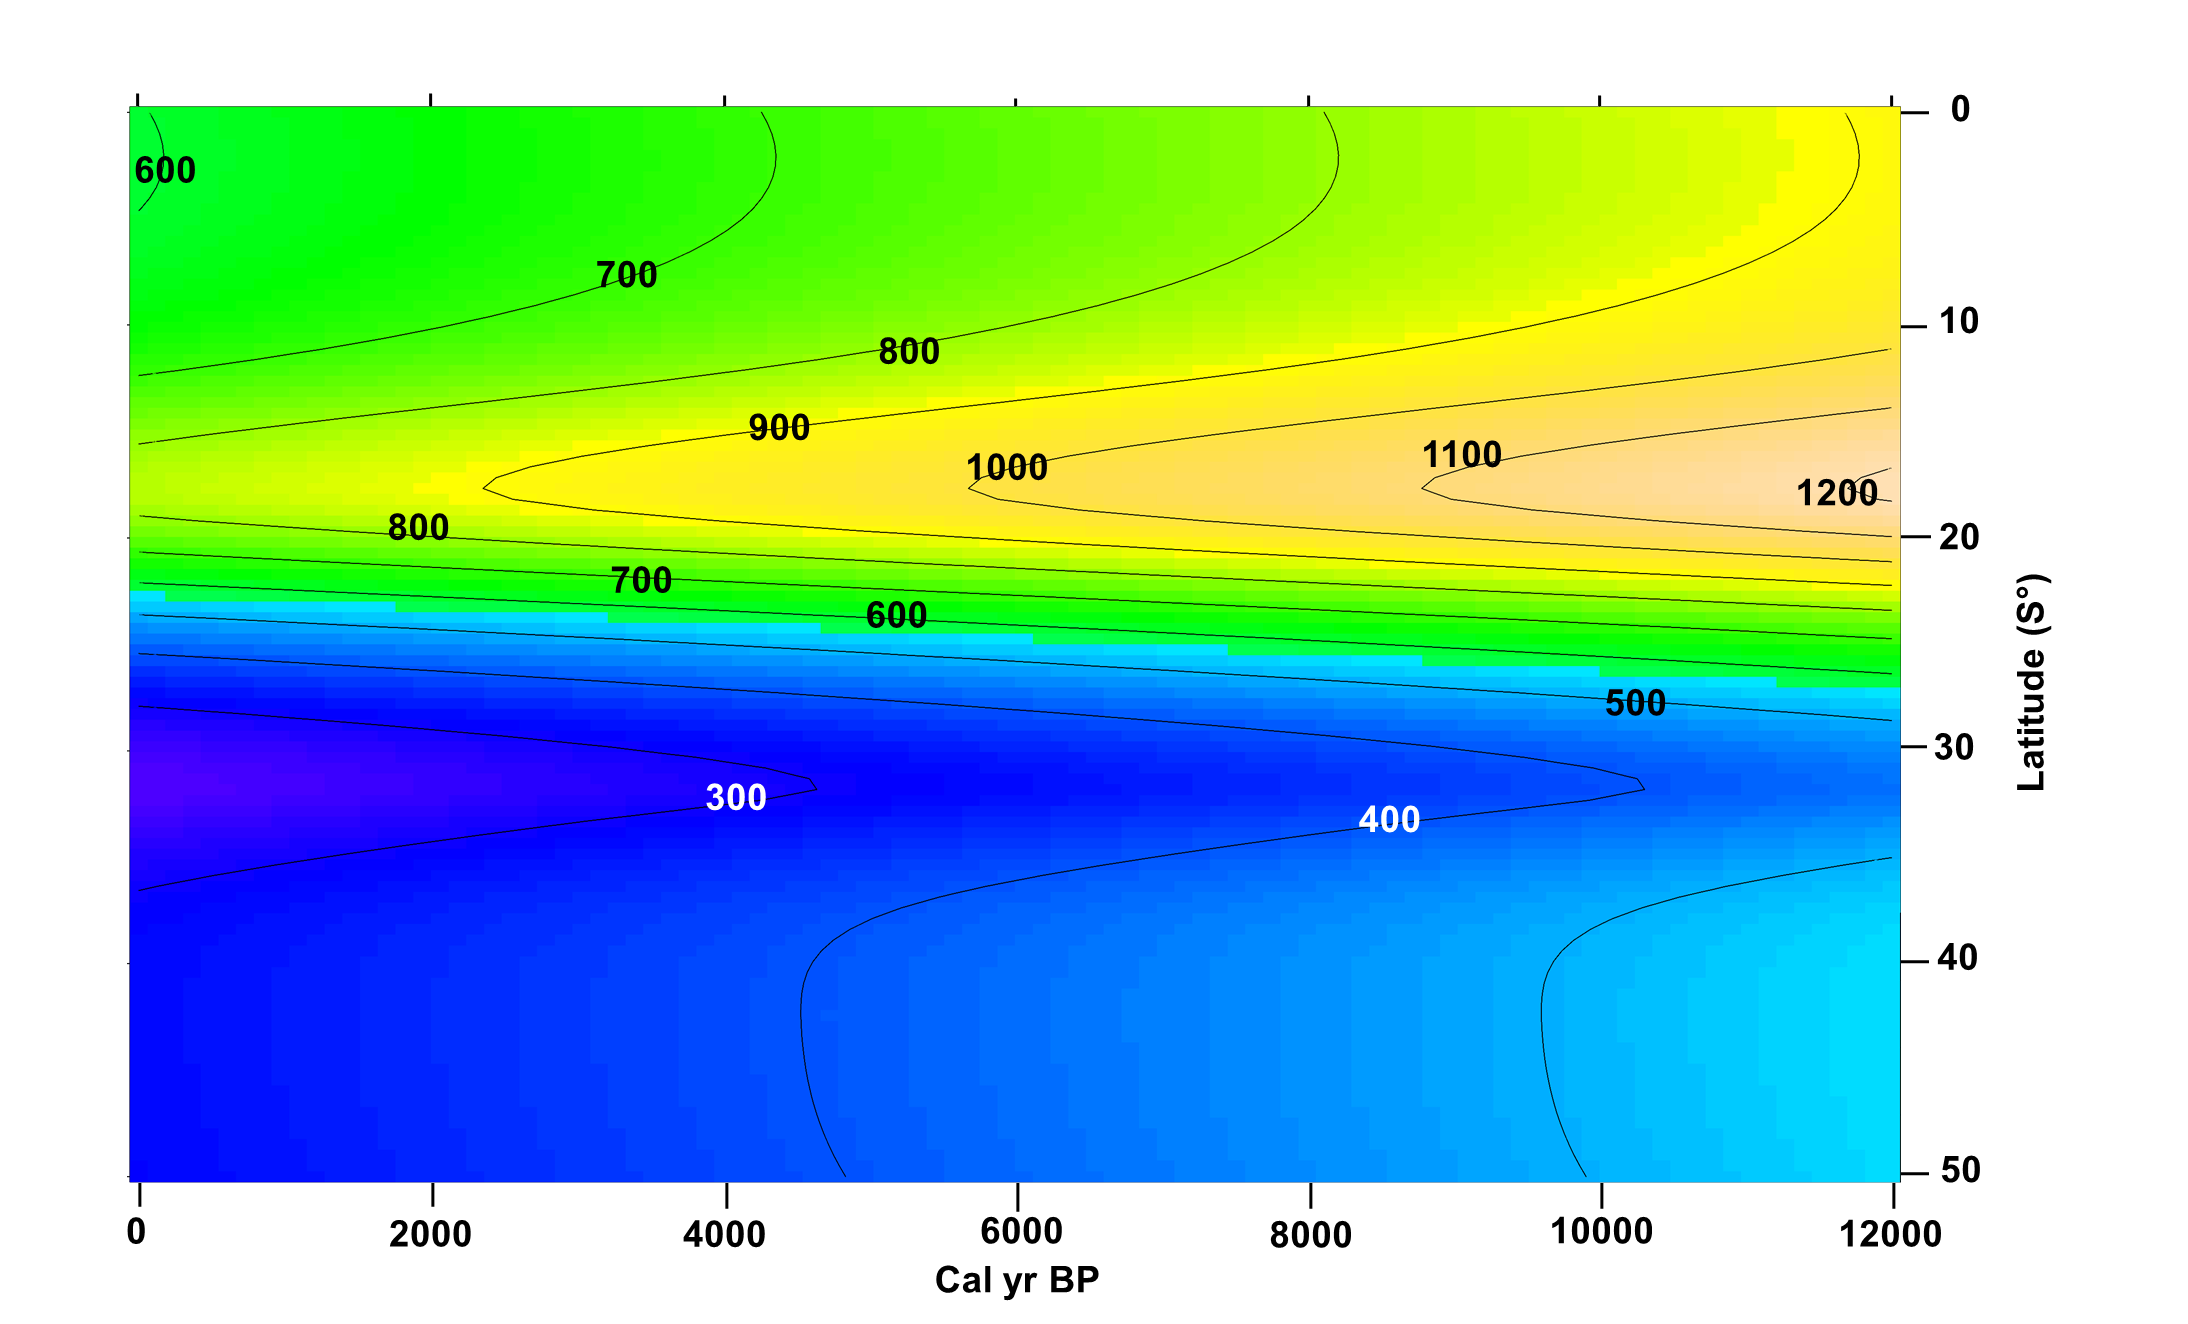
\includegraphics{GAM radiocarbon heat map.png}}
\end{minipage} \\
\midrule
\endhead
\emph{Figure 3. Latitudinal distribution of MRA off Peru \& Chile the
last 12 Kyr BP} \\
\bottomrule
\end{longtable}

Then, I plotted a scatter of MRA, regarding calibrated age and latitude
according to GAM
\protect\hyperlink{latitudinal-distribution-of-mra}{(fig.~3)}. this
picture I can see a sharp latitudinal pattern in two zones: first (O to
22°S) and second (22 to 50°S). the border between two zones could be
displacement northward during the last 12 Kyr BP.

\hypertarget{mra-estimated-under-marine20}{%
\subsubsection{MRA estimated under
Marine20}\label{mra-estimated-under-marine20}}

At the state above the latitudinal pattern of MRA in two zones is
reliably acceptable. Accordingly, I can estimate an MRA by latitude and
periods of time, similar to previous works
\protect\hyperlink{mra-estimated-under-marine20}{(fig.~4)}.

\begin{longtable}[]{@{}
  >{\centering\arraybackslash}p{(\columnwidth - 0\tabcolsep) * \real{1.0000}}@{}}
\toprule
\begin{minipage}[b]{\linewidth}\centering
\href{https://github.com/jasb3110/Radiocarbon-reservoir/blob/db842ff0620d55ea5ca5ceec0d96a369406b6e3c/MRA.marine20.png?raw=true}{\includegraphics{MRA.marine20.png}}
\end{minipage} \\
\midrule
\endhead
\emph{Figure 4. Diagram of local Marine reservoir age off Peru \& Chile
in boxes. Diagram of local Marine reservoir age off Peru \& Chile in
boxes. Orange boxes belonged from 0 to 22°S and purple boxes belonged
from 22 to 50°S.The thick black lines is mean value of MRA each box.} \\
\bottomrule
\end{longtable}

In this picture, I show the estimation of local MRA in boxes. for two
zones, Calibrated age of MRA does not belong same time windows. There
are four boxes (two orange and two purple) boxes of MRA that have
belonged to different latitudinal positions and periods of time (orange
boxes: latitude 0-22°S, 10.6 to 5.8 Kyr BP and 5.6 to 0.3 Kyr BP; purple
boxes: latitude 22-50°S, 12 to 6.5 Kyr BP and 3.4 to 0.1 Kyr BP).

\hypertarget{discussion}{%
\subsection{Discussion}\label{discussion}}

\begin{longtable}[]{@{}
  >{\centering\arraybackslash}p{(\columnwidth - 0\tabcolsep) * \real{1.0000}}@{}}
\toprule
\begin{minipage}[b]{\linewidth}\centering
\href{https://github.com/jasb3110/Radiocarbon-reservoir/blob/8bddc9b0f2d8f839ca2d4826f47d9050d49384aa/animation.gif?raw=true}{\includegraphics{animation.gif?}}
\end{minipage} \\
\midrule
\endhead
\emph{Figure 5.Animation of local MRA off Peru \& Chile in boxes.Global
of MRA estimated for each calibrated curve how to difference between
Scal2013 \& Marine2013 (grey) and Scal2020 \& Marine2020(red). Estimated
local of MRA by Ortlieb et al.~2011(grey); by Carré et al.~2016(green
and blue) and by this work(orange and purple).The thick black lines is
mean value of MRA each box} \\
\bottomrule
\end{longtable}

\hypertarget{conclusions}{%
\subsection{Conclusions}\label{conclusions}}

\hypertarget{references}{%
\subsection{References}\label{references}}

\hypertarget{r-code}{%
\subsection{R code}\label{r-code}}

Bellow I attached a R-script.
\href{mailto:solisbenites.jose@gmail.com}{Contact Us} here, if you
consider to give opinions, suggestions and questions.

\begin{Shaded}
\begin{Highlighting}[]
\NormalTok{\#\#\#\#\#\#\#\#\#\#\#\#\#\#\#\#\#\#\#\#\#\#\#\#\#\#\#\#\#\#\#\#\#\#\#\#\#\#\#\#\#\#\#\#\#\#\#\#\#\#\#\#\#\#\#\#\#\#\#\#\#\#\#\#\#\#\#\#\#\#\#\#\#\#\#\#\#\#\#\#}
\NormalTok{\#to start}

\NormalTok{setwd("\textasciitilde{}/Radiocarbon{-}reservoir/")\#directory}

\NormalTok{library("Bchron")}

\NormalTok{\#To delete outliers}
\NormalTok{d=read.csv("Radiocarbon reservoir.csv",sep=";",dec=".",header = TRUE)\#data all data}
\NormalTok{d=as.data.frame(d)}
\NormalTok{d$label=paste(d$reference,d$latitude,"°","{-}Material:",d$type.of.material,"Sample:",d$pair,sep=" ")}
\NormalTok{d$curve=d$calibrate.curve}
\NormalTok{d$curve}\CommentTok{[}\OtherTok{d$calibrate.curve=="terrestrial"\&d$Convencial.age\textgreater{}=126}\CommentTok{]}\NormalTok{="shcal20"\#155 ± 11 BP (Hogg et al. 2019) is used in SHCal20.}
\NormalTok{d$curve}\CommentTok{[}\OtherTok{d$calibrate.curve=="marine"}\CommentTok{]}\NormalTok{="Marine20"}
\NormalTok{d$curve}\CommentTok{[}\OtherTok{which(d$calibrate.curve=="terrestrial"\&d$Convencial.age\textless{}126)}\CommentTok{]}\NormalTok{="normal"}
\NormalTok{d$Convencial.age}\CommentTok{[}\OtherTok{which(d$calibrate.curve=="marine"\&d$Convencial.age\textless{}603)}\CommentTok{]}\NormalTok{=604}

\NormalTok{age.t=BchronCalibrate( \#It is getting calibrated in Marine20 and Shcal20}
\NormalTok{  ages = d$Convencial.age,}
\NormalTok{  ageSds = d$SD.convencial.age,}
\NormalTok{  eps = 1e{-}05,}
\NormalTok{  calCurves =d$curve,}
\NormalTok{  positions = d$latitude,}
\NormalTok{  ids=d$label)}

\NormalTok{hafsigma=.382924922548026\#0.382924922548026 }
\NormalTok{onesigma=.682689492137086\#0.682689492137086}
\NormalTok{twosigma=.954499736103642\#0.954499736103642}

\NormalTok{\#p=hafsigma\# half sigma}
\NormalTok{\#p=onesigma\#one sigma}
\NormalTok{p=twosigma\#two sigma}

\NormalTok{d$lower=NULL}
\NormalTok{d$upper=NULL}
\NormalTok{d$max=NULL}
\NormalTok{d$median=NULL}

\NormalTok{vvv=NULL}
\NormalTok{sss=NULL}

\NormalTok{for (i in 1:dim(d)}\CommentTok{[}\OtherTok{1}\CommentTok{]}\NormalTok{)\{}
\NormalTok{  d$mean}\CommentTok{[}\OtherTok{i}\CommentTok{]}\NormalTok{=sum(age.t[}\CommentTok{[}\OtherTok{i}\CommentTok{]}\NormalTok{]$densities*age.t[}\CommentTok{[}\OtherTok{i}\CommentTok{]}\NormalTok{]$ageGrid)}
\NormalTok{  d$median}\CommentTok{[}\OtherTok{i}\CommentTok{]}\NormalTok{=age.t[}\CommentTok{[}\OtherTok{i}\CommentTok{]}\NormalTok{]$ageGrid}\CommentTok{[}\OtherTok{round(length(age.t[[i]}\CommentTok{]}\NormalTok{$densities)*0.5)]}
  
\NormalTok{  if(length(age.t[}\CommentTok{[}\OtherTok{i}\CommentTok{]}\NormalTok{]$ageGrid}\CommentTok{[}\OtherTok{which(age.t[[i]}\CommentTok{]}\NormalTok{$densities==max(age.t[}\CommentTok{[}\OtherTok{i}\CommentTok{]}\NormalTok{]$densities))])==1)\{}
\NormalTok{  d$max}\CommentTok{[}\OtherTok{i}\CommentTok{]}\NormalTok{=age.t[}\CommentTok{[}\OtherTok{i}\CommentTok{]}\NormalTok{]$ageGrid}\CommentTok{[}\OtherTok{which(age.t[[i]}\CommentTok{]}\NormalTok{$densities==max(age.t[}\CommentTok{[}\OtherTok{i}\CommentTok{]}\NormalTok{]$densities))]}
\NormalTok{  \}else\{}
\NormalTok{    vvv=age.t[}\CommentTok{[}\OtherTok{i}\CommentTok{]}\NormalTok{]$ageGrid}\CommentTok{[}\OtherTok{which(age.t[[i]}\CommentTok{]}\NormalTok{$densities==max(age.t[}\CommentTok{[}\OtherTok{i}\CommentTok{]}\NormalTok{]$densities))]}
\NormalTok{    sss= abs(vvv{-}d$mean}\CommentTok{[}\OtherTok{i}\CommentTok{]}\NormalTok{)}
\NormalTok{  d$max}\CommentTok{[}\OtherTok{i}\CommentTok{]}\NormalTok{= vvv}\CommentTok{[}\OtherTok{which(sss==min(sss))}\CommentTok{]}
\NormalTok{  \}}
  
\NormalTok{  if(max(age.t[}\CommentTok{[}\OtherTok{i}\CommentTok{]}\NormalTok{]$ageGrid}\CommentTok{[}\OtherTok{which(cumsum(age.t[[i]}\CommentTok{]}\NormalTok{$densities)\textless{}cumsum(age.t[}\CommentTok{[}\OtherTok{i}\CommentTok{]}\NormalTok{]$densities)}\CommentTok{[}\OtherTok{which(age.t[[i]}\CommentTok{]}\NormalTok{$ageGrid==d$max}\CommentTok{[}\OtherTok{i}\CommentTok{]}\NormalTok{)]{-}p*.5)])=={-}Inf)\{}
\NormalTok{  d$upper}\CommentTok{[}\OtherTok{i}\CommentTok{]}\NormalTok{=min(age.t[}\CommentTok{[}\OtherTok{i}\CommentTok{]}\NormalTok{]$ageGrid)  }
\NormalTok{  \}else\{}
\NormalTok{  d$upper}\CommentTok{[}\OtherTok{i}\CommentTok{]}\NormalTok{=max(age.t[}\CommentTok{[}\OtherTok{i}\CommentTok{]}\NormalTok{]$ageGrid}\CommentTok{[}\OtherTok{which(cumsum(age.t[[i]}\CommentTok{]}\NormalTok{$densities)\textless{}cumsum(age.t[}\CommentTok{[}\OtherTok{i}\CommentTok{]}\NormalTok{]$densities)}\CommentTok{[}\OtherTok{which(age.t[[i]}\CommentTok{]}\NormalTok{$ageGrid==d$max}\CommentTok{[}\OtherTok{i}\CommentTok{]}\NormalTok{)]{-}p*.5)])}
\NormalTok{  \}}
  
\NormalTok{  if(min(age.t[}\CommentTok{[}\OtherTok{i}\CommentTok{]}\NormalTok{]$ageGrid}\CommentTok{[}\OtherTok{which(cumsum(age.t[[i]}\CommentTok{]}\NormalTok{$densities)\textgreater{}cumsum(age.t[}\CommentTok{[}\OtherTok{i}\CommentTok{]}\NormalTok{]$densities)}\CommentTok{[}\OtherTok{which(age.t[[i]}\CommentTok{]}\NormalTok{$ageGrid==d$max}\CommentTok{[}\OtherTok{i}\CommentTok{]}\NormalTok{)]+p*.5)])==Inf)\{}
\NormalTok{  d$lower}\CommentTok{[}\OtherTok{i}\CommentTok{]}\NormalTok{=max(age.t[}\CommentTok{[}\OtherTok{i}\CommentTok{]}\NormalTok{]$ageGrid) }
\NormalTok{  \}else\{}
\NormalTok{  d$lower}\CommentTok{[}\OtherTok{i}\CommentTok{]}\NormalTok{=min(age.t[}\CommentTok{[}\OtherTok{i}\CommentTok{]}\NormalTok{]$ageGrid}\CommentTok{[}\OtherTok{which(cumsum(age.t[[i]}\CommentTok{]}\NormalTok{$densities)\textgreater{}cumsum(age.t[}\CommentTok{[}\OtherTok{i}\CommentTok{]}\NormalTok{]$densities)}\CommentTok{[}\OtherTok{which(age.t[[i]}\CommentTok{]}\NormalTok{$ageGrid==d$max}\CommentTok{[}\OtherTok{i}\CommentTok{]}\NormalTok{)]+p*.5)])}
\NormalTok{  \}}
\NormalTok{  \}}

\NormalTok{d$sdmean.lower=abs(d$lower{-}d$mean)}
\NormalTok{d$sdmean.upper=abs(d$mean{-}d$upper)}

\NormalTok{d$sdmedian.lower=abs(d$lower{-}d$median)}
\NormalTok{d$sdmedian.upper=abs(d$median{-}d$upper)}

\NormalTok{d$sdmax.lower=abs(d$lower{-}d$max)}
\NormalTok{d$sdmax.upper=abs(d$max{-}d$upper)}

\NormalTok{\#for (i in 1:dim(d)}\CommentTok{[}\OtherTok{1}\CommentTok{]}\NormalTok{)\{}
\NormalTok{\#X11();plot(age.t[}\CommentTok{[}\OtherTok{i}\CommentTok{]}\NormalTok{]$ageGrid,age.t[}\CommentTok{[}\OtherTok{i}\CommentTok{]}\NormalTok{]$densities,type="l",xlab="Cal BP",ylab="Density",main =d$label}\CommentTok{[}\OtherTok{i}\CommentTok{]}\NormalTok{)}
\NormalTok{\#abline(v=d$mean}\CommentTok{[}\OtherTok{i}\CommentTok{]}\NormalTok{,col="gray")\#mean value}
\NormalTok{\#abline(v=d$lower}\CommentTok{[}\OtherTok{i}\CommentTok{]}\NormalTok{,col="blue")\# lower value}
\NormalTok{\#abline(v=d$upper}\CommentTok{[}\OtherTok{i}\CommentTok{]}\NormalTok{,col="red")\#upper value}
\NormalTok{\#abline(v=d$median}\CommentTok{[}\OtherTok{i}\CommentTok{]}\NormalTok{,col="green")\#median value}
\NormalTok{\#abline(v=d$max}\CommentTok{[}\OtherTok{i}\CommentTok{]}\NormalTok{,col="black")\#Maximum probability value, this was useful!}
\NormalTok{\#}

\NormalTok{\#\#\#\#\#\#\#\#\#\#\#\#\#\#\#\#\#\#\#\#\#\#\#\#\#\#\#\#\#\#\#\#\#\#\#\#\#\#\#\#\#\#\#\#\#\#\#\#\#\#\#\#\#\#\#\#\#\#\#\#\#\#\#\#\#\#\#\#\#\#\#\#\#\#\#\#\#\#\#\#}
\NormalTok{\#According to Russel et al.2011}
\NormalTok{\#density of R is estimated for bootstrapping ("n")}

\NormalTok{n=1000000\# 1 millon resamples!}

\NormalTok{  funclist=list()}
\NormalTok{  for(i in 1:dim(d)}\CommentTok{[}\OtherTok{1}\CommentTok{]}\NormalTok{)\{}
\NormalTok{    funclist[}\CommentTok{[}\OtherTok{i}\CommentTok{]}\NormalTok{]=assign(paste0("funt",i),approxfun(density(age.t[}\CommentTok{[}\OtherTok{i}\CommentTok{]}\NormalTok{]$densities)))}
\NormalTok{    assign(paste0(d$calibrate.curve}\CommentTok{[}\OtherTok{i}\CommentTok{]}\NormalTok{,i),sample(x=age.t[}\CommentTok{[}\OtherTok{i}\CommentTok{]}\NormalTok{]$ageGrid}\CommentTok{[}\OtherTok{1:length(age.t[[i]}\CommentTok{]}\NormalTok{$densities)],}
\NormalTok{                                                 size =n,}
\NormalTok{                                                 replace=TRUE,}
\NormalTok{                                                 prob = funclist[}\CommentTok{[}\OtherTok{i}\CommentTok{]}\NormalTok{](age.t[}\CommentTok{[}\OtherTok{i}\CommentTok{]}\NormalTok{]$densities}\CommentTok{[}\OtherTok{1:length(age.t[[i]}\CommentTok{]}\NormalTok{$densities)])))}
\NormalTok{  \}}

\NormalTok{d$calibrate.curve}\CommentTok{[}\OtherTok{d$calibrate.curve=="normal"}\CommentTok{]}\NormalTok{="terrestrial"}

\NormalTok{\#\#\#\#\#\#\#\#\#\#\#\#\#\#\#\#\#\#\#\#\#\#\#\#\#\#\#\#\#\#\#\#\#\#\#\#\#\#\#\#\#\#\#\#\#\#\#\#\#\#\#\#\#\#\#\#\#\#\#\#\#\#\#\#\#\#\#\#\#\#\#\#\#\#\#\#\#\#\#\#}
\NormalTok{\#Estimated Radiocarbon reservoir effect each sample}
\NormalTok{\#samples}

\NormalTok{rlist=list()}
\NormalTok{sec=seq(2,dim(d)}\CommentTok{[}\OtherTok{1}\CommentTok{]}\NormalTok{,2)}

\NormalTok{for(i in sec)\{}
\NormalTok{  rlist[}\CommentTok{[}\OtherTok{i}\CommentTok{]}\NormalTok{]=assign(paste0("r",i*.5),get(paste0("marine",i{-}1)){-}get(paste0("terrestrial",i)))}
\NormalTok{\}}

\NormalTok{t.r=as.data.frame(cbind(as.numeric(d$latitude}\CommentTok{[}\OtherTok{sec}\CommentTok{]}\NormalTok{),as.numeric(d$longitude}\CommentTok{[}\OtherTok{sec}\CommentTok{]}\NormalTok{),d$max}\CommentTok{[}\OtherTok{sec}\CommentTok{]}\NormalTok{,d$sdmax.lower}\CommentTok{[}\OtherTok{sec}\CommentTok{]}\NormalTok{*.5+d$sdmax.upper[sec]*.5,NA,NA,d$pairs}\CommentTok{[}\OtherTok{sec}\CommentTok{]}\NormalTok{,d$reference}\CommentTok{[}\OtherTok{sec}\CommentTok{]}\NormalTok{,d$obs}\CommentTok{[}\OtherTok{sec}\CommentTok{]}\NormalTok{,d$period.time}\CommentTok{[}\OtherTok{sec}\CommentTok{]}\NormalTok{))}

\NormalTok{colnames(t.r)=c("latitude","longitude","Cal BP(Maximun probability)","error(yr)","R","sdR","pair","reference","obs","period")}

\NormalTok{for(i in 1:length(t.r$latitude))\{}
\NormalTok{t.r$R}\CommentTok{[}\OtherTok{i}\CommentTok{]}\NormalTok{=as.numeric(round(mean(get(paste0("r",i))),2))}
\NormalTok{t.r$sdR}\CommentTok{[}\OtherTok{i}\CommentTok{]}\NormalTok{=as.numeric(round(sd(get(paste0("r",i))),2))}
\NormalTok{\}}

\NormalTok{label=paste0(t.r$latitude,"/",t.r$}\InformationTok{\textasciigrave{}Cal BP(Maximun probability)\textasciigrave{}}\NormalTok{,"/",t.r$longitude)}
\NormalTok{label=factor(label,levels=unique(label))}
\NormalTok{t.r$label=label}

\NormalTok{write.csv(t.r,"outcome.csv",sep=";",dec=".",col.names = TRUE) }
\NormalTok{\#\#\#\#\#\#\#\#\#\#\#\#\#\#\#\#\#\#\#\#\#\#\#\#\#\#\#\#\#\#\#\#\#\#\#\#\#\#\#\#\#\#\#\#\#\#\#\#\#\#\#\#\#\#\#\#\#\#\#\#\#\#\#\#\#\#\#\#\#\#\#\#\#\#\#\#\#\#\#}
\NormalTok{\#Method of Error propagation of variance, according to R.Reimer \& P.Reimer et al. 2016}
\NormalTok{\#Asumption three sample is minimum of pool database}
\NormalTok{\#I create a function Error in the weighted mean().}

\NormalTok{error.weigthed.mean=function(r,dr,sigma=2,show=1,warning=0,...)\{}
\NormalTok{  if(is.numeric(r)\&\&is.numeric(dr)!=1)\{}
\NormalTok{    stop("Vector values is/are not number(s)") }
\NormalTok{  \}else\{  }
\NormalTok{    if(sum(is.na(r)+is.na(dr))\textgreater{}0)\{}
\NormalTok{      stop("Vector values has NAs") }
\NormalTok{    \}else\{ }
\NormalTok{      if(length(r)/length(dr)!=1)\{ }
\NormalTok{        stop("Vector values are not same size") }
\NormalTok{      \}else\{}
\NormalTok{        if(sum(sigma\textless{}5\&sigma\textgreater{}0)==0)\{}
\NormalTok{          stop("sigma is a value should be major 0 and less 5")}
\NormalTok{        \}else\{}
\NormalTok{          if(length(r)==1)\{}
\NormalTok{            rm=r}
\NormalTok{            delta.r=dr}
\NormalTok{            warn.sign="There is one value, suggesting aggregate more values"}
\NormalTok{          \}else\{    }
\NormalTok{          if(length(r)==2)\{}
\NormalTok{            rm=sum(r/dr\^{}2)/sum( 1/dr\^{}2)}
\NormalTok{            delta.r=sigma*sqrt(1/sum(1/dr\^{}2))}
\NormalTok{            warn.sign="There are two values, suggesting aggregate more values"}
\NormalTok{          \}else\{}
\NormalTok{            rm=sum(r/dr\^{}2)/sum( 1/dr\^{}2)}
\NormalTok{            delta.r =sigma*sqrt((sum(((r{-}rm)/dr)\^{}2)/(length(r){-}1))/(sum((1/dr)\^{}2)/length(r)))}
\NormalTok{            warn.sign=NULL}
\NormalTok{          \}}
\NormalTok{        \}}
\NormalTok{      \}}
\NormalTok{    \}}
\NormalTok{    \}}
\NormalTok{  \}}

\NormalTok{if(sum(warning==TRUE,warning==FALSE,warning==T,warning==F,warning==1,warning==0)==0)\{}
\NormalTok{    stop("if you would see warning: TRUE or T or 1 if you not: FALSE or F or 0") }
\NormalTok{  \}else\{  }
\NormalTok{    if(show==TRUE)\{}
\NormalTok{      print(warn.sign)}
\NormalTok{    \}else\{}
\NormalTok{      invisible()}
\NormalTok{    \}}
\NormalTok{  \}}

\NormalTok{if(sum(show==TRUE,show==FALSE,show==T,show==F,show==1,show==0)==0)\{}
\NormalTok{  stop("if you would see results: TRUE or T or 1 if you not: FALSE or F or 0") }
\NormalTok{  \}else\{  }
\NormalTok{    if(show==TRUE)\{}
\NormalTok{      print(paste0("Mean of Reservoir effect is ",round(rm,0)," and Uncertainty of Reservoir effect is ",round(delta.r,0)))}
\NormalTok{    \}else\{}
\NormalTok{      invisible()}
\NormalTok{    \}}
\NormalTok{  \}}
\NormalTok{outcome=c(rm,delta.r)}
\NormalTok{invisible(outcome)  }
\NormalTok{\}}
\NormalTok{\#\#\#\#\#\#\#\#\#\#\#\#\#\#\#\#\#\#\#\#\#\#\#\#\#\#\#\#\#\#\#\#\#\#\#\#\#\#\#\#\#\#\#\#\#\#\#\#\#\#\#\#\#\#\#\#\#\#\#\#\#\#\#\#\#\#\#\#\#\#\#\#\#\#\#\#\#\#\#}
\NormalTok{\#to reduce a repeated samples, so that it decrease overweight.}
\NormalTok{\#Then repeated samples are merged according error.weigthed.mean function.}
\NormalTok{p2=unique(t.r$label)}
\NormalTok{t.r2=t.r}\CommentTok{[}\OtherTok{1:length(p2),}\CommentTok{]}
\NormalTok{t.r2}\CommentTok{[}\OtherTok{1:length(p2),}\CommentTok{]}\NormalTok{=NA}
\NormalTok{t.r2$label=p2}

\NormalTok{for(i in 1:length(p2))\{}
\NormalTok{t.r2$latitude}\CommentTok{[}\OtherTok{i}\CommentTok{]}\NormalTok{=t.r$latitude}\CommentTok{[}\OtherTok{which(t.r$label==t.r2$label[i])}\CommentTok{][1]}
\NormalTok{t.r2$longitude}\CommentTok{[}\OtherTok{i}\CommentTok{]}\NormalTok{= t.r$longitude}\CommentTok{[}\OtherTok{which(t.r$label==t.r2$label[i])}\CommentTok{][1]} 
\NormalTok{t.r2$reference}\CommentTok{[}\OtherTok{i}\CommentTok{]}\NormalTok{=t.r$reference}\CommentTok{[}\OtherTok{which(t.r$label==t.r2$label[i])}\CommentTok{][1]} 
\NormalTok{t.r2$obs}\CommentTok{[}\OtherTok{i}\CommentTok{]}\NormalTok{=t.r$obs}\CommentTok{[}\OtherTok{which(t.r$label==t.r2$label[i])}\CommentTok{][1]} 
\NormalTok{t.r2$pair}\CommentTok{[}\OtherTok{i}\CommentTok{]}\NormalTok{=t.r$pair}\CommentTok{[}\OtherTok{which(t.r$label==t.r2$label[i])}\CommentTok{][1]} 
\NormalTok{t.r2$period}\CommentTok{[}\OtherTok{i}\CommentTok{]}\NormalTok{=t.r$period}\CommentTok{[}\OtherTok{which(t.r$label==t.r2$label[i])}\CommentTok{][1]} 
\NormalTok{t.r2$}\InformationTok{\textasciigrave{}Cal BP(Maximun probability)\textasciigrave{}}\CommentTok{[}\OtherTok{i}\CommentTok{]}\NormalTok{=t.r$}\InformationTok{\textasciigrave{}Cal BP(Maximun probability)\textasciigrave{}}\CommentTok{[}\OtherTok{which(t.r$label==t.r2$label[i])}\CommentTok{][1]} 
\NormalTok{t.r2$}\InformationTok{\textasciigrave{}error(yr)\textasciigrave{}}\CommentTok{[}\OtherTok{i}\CommentTok{]}\NormalTok{=t.r$}\InformationTok{\textasciigrave{}error(yr)\textasciigrave{}}\CommentTok{[}\OtherTok{which(t.r$label==t.r2$label[i])}\CommentTok{][1]} 
\NormalTok{t.r2$R}\CommentTok{[}\OtherTok{i}\CommentTok{]}\NormalTok{=error.weigthed.mean(as.numeric(t.r$R}\CommentTok{[}\OtherTok{which(t.r$label==t.r2$label[i])}\CommentTok{]}\NormalTok{),dr=as.numeric(t.r$sdR}\CommentTok{[}\OtherTok{which(t.r$label==t.r2$label[i])}\CommentTok{]}\NormalTok{),sigma = 1,show = 0,warning = 0)}\CommentTok{[}\OtherTok{1}\CommentTok{]}
\NormalTok{t.r2$sdR}\CommentTok{[}\OtherTok{i}\CommentTok{]}\NormalTok{=error.weigthed.mean(as.numeric(t.r$R}\CommentTok{[}\OtherTok{which(t.r$label==t.r2$label[i])}\CommentTok{]}\NormalTok{),dr=as.numeric(t.r$sdR}\CommentTok{[}\OtherTok{which(t.r$label==t.r2$label[i])}\CommentTok{]}\NormalTok{),sigma = 1,show = 0,warning = 0)}\CommentTok{[}\OtherTok{2}\CommentTok{]}
\NormalTok{\}}

\NormalTok{t.r2$label=NULL}

\NormalTok{write.csv(t.r2,"outcome2.csv",sep=";",dec=".",col.names = TRUE)  }

\NormalTok{\#\#\#\#\#\#\#\#\#\#\#\#\#\#\#\#\#\#\#\#\#\#\#\#\#\#\#\#\#\#\#\#\#\#\#\#\#\#\#\#\#\#\#\#\#\#\#\#\#\#\#\#\#\#\#\#\#\#\#\#\#\#\#\#\#\#\#\#\#\#\#\#\#\#\#\#\#\#\#}
\FunctionTok{\# To estimate of Radiocarbon reservoir effect on Boxes.}

\NormalTok{\#for latitude 0°S{-}22°S during 6000 to 10500 yr BP}
\NormalTok{w={-}22}
\NormalTok{sigma1=2}
\NormalTok{showme=1}
\NormalTok{warn=1}

\NormalTok{Rp1=as.numeric(t.r2$R}\CommentTok{[}\OtherTok{as.numeric(t.r2$latitude)\textgreater{}w\&as.numeric(t.r2$\textasciigrave{}Cal BP(Maximun probability)\textasciigrave{})\textgreater{}6000\&t.r2$obs!="not relationship"}\CommentTok{]}\NormalTok{)}
\NormalTok{sRp1=as.numeric(t.r2$sdR}\CommentTok{[}\OtherTok{as.numeric(t.r2$latitude)\textgreater{}w\&as.numeric(t.r2$\textasciigrave{}Cal BP(Maximun probability)\textasciigrave{})\textgreater{}6000\&t.r2$obs!="not relationship"}\CommentTok{]}\NormalTok{)}
\NormalTok{c1=as.numeric(t.r2$}\InformationTok{\textasciigrave{}Cal BP(Maximun probability)\textasciigrave{}}\CommentTok{[}\OtherTok{as.numeric(t.r2$latitude)\textgreater{}w\&as.numeric(t.r2$\textasciigrave{}Cal BP(Maximun probability)\textasciigrave{})\textgreater{}6000\&t.r2$obs!="not relationship"}\CommentTok{]}\NormalTok{)}
\NormalTok{p1=error.weigthed.mean(Rp1,sRp1,sigma1,showme,warn)}

\NormalTok{\#during 100 to 5500 yr BP}
\NormalTok{Rp2=as.numeric(t.r2$R}\CommentTok{[}\OtherTok{as.numeric(t.r2$latitude)\textgreater{}w\&as.numeric(t.r2$\textasciigrave{}Cal BP(Maximun probability)\textasciigrave{})\textgreater{}100\&as.numeric(t.r2$\textasciigrave{}Cal BP(Maximun probability)\textasciigrave{})\textless{}5500\&t.r2$obs!="not relationship"}\CommentTok{]}\NormalTok{)}
\NormalTok{sRp2=as.numeric(t.r2$sdR}\CommentTok{[}\OtherTok{as.numeric(t.r2$latitude)\textgreater{}w\&as.numeric(t.r2$\textasciigrave{}Cal BP(Maximun probability)\textasciigrave{})\textgreater{}100\&as.numeric(t.r2$\textasciigrave{}Cal BP(Maximun probability)\textasciigrave{})\textless{}5500\&t.r2$obs!="not relationship"}\CommentTok{]}\NormalTok{)}
\NormalTok{c2=as.numeric(t.r2$}\InformationTok{\textasciigrave{}Cal BP(Maximun probability)\textasciigrave{}}\CommentTok{[}\OtherTok{as.numeric(t.r2$latitude)\textgreater{}w\&as.numeric(t.r2$\textasciigrave{}Cal BP(Maximun probability)\textasciigrave{})\textgreater{}100\&as.numeric(t.r2$\textasciigrave{}Cal BP(Maximun probability)\textasciigrave{})\textless{}5500\&t.r2$obs!="not relationship"}\CommentTok{]}\NormalTok{)}
\NormalTok{p2=error.weigthed.mean(Rp2,sRp2,sigma1,showme,warn)}

\NormalTok{\#during 100 to 4000 yr BP}
\NormalTok{\#Rp3=as.numeric(t.r2$R}\CommentTok{[}\OtherTok{as.numeric(t.r2$latitude)\textgreater{}w\&as.numeric(t.r2$\textasciigrave{}Cal BP(Maximun probability)\textasciigrave{})\textgreater{}100\&as.numeric(t.r2$\textasciigrave{}Cal BP(Maximun probability)\textasciigrave{})\textless{}4000\&t.r2$obs!="not relationship"}\CommentTok{]}\NormalTok{)}
\NormalTok{\#sRp3=as.numeric(t.r2$sdR}\CommentTok{[}\OtherTok{as.numeric(t.r2$latitude)\textgreater{}w\&as.numeric(t.r2$\textasciigrave{}Cal BP(Maximun probability)\textasciigrave{})\textgreater{}100\&as.numeric(t.r2$\textasciigrave{}Cal BP(Maximun probability)\textasciigrave{})\textless{}4000\&t.r2$obs!="not relationship"}\CommentTok{]}\NormalTok{)}
\NormalTok{\#error.weigthed.mean(Rp3,sRp3,sigma1,showme,warn)}

\NormalTok{\#during {-}10 to 100 yr BP}
\NormalTok{Rp4=as.numeric(t.r2$R}\CommentTok{[}\OtherTok{as.numeric(t.r2$latitude)\textgreater{}w\&as.numeric(t.r2$\textasciigrave{}Cal BP(Maximun probability)\textasciigrave{})\textgreater{}{-}10\&as.numeric(t.r2$\textasciigrave{}Cal BP(Maximun probability)\textasciigrave{})\textless{}100\&t.r2$obs!="not relationship"}\CommentTok{]}\NormalTok{)}
\NormalTok{sRp4=as.numeric(t.r2$sdR}\CommentTok{[}\OtherTok{as.numeric(t.r2$latitude)\textgreater{}w\&as.numeric(t.r2$\textasciigrave{}Cal BP(Maximun probability)\textasciigrave{})\textgreater{}{-}10\&as.numeric(t.r2$\textasciigrave{}Cal BP(Maximun probability)\textasciigrave{})\textless{}100\&t.r2$obs!="not relationship"}\CommentTok{]}\NormalTok{)}
\NormalTok{c3=as.numeric(t.r2$}\InformationTok{\textasciigrave{}Cal BP(Maximun probability)\textasciigrave{}}\CommentTok{[}\OtherTok{as.numeric(t.r2$latitude)\textgreater{}w\&as.numeric(t.r2$\textasciigrave{}Cal BP(Maximun probability)\textasciigrave{})\textgreater{}{-}10\&as.numeric(t.r2$\textasciigrave{}Cal BP(Maximun probability)\textasciigrave{})\textless{}100\&t.r2$obs!="not relationship"}\CommentTok{]}\NormalTok{)}
\NormalTok{p3=error.weigthed.mean(Rp4,sRp4,sigma1,showme,warn)}

\NormalTok{\#for latitude{-}22°S{-}51°S}
\NormalTok{\#during 6000 to 10500 yr BP}
\NormalTok{Rp5=as.numeric(t.r2$R}\CommentTok{[}\OtherTok{as.numeric(t.r2$latitude)\textless{}w\&as.numeric(t.r2$\textasciigrave{}Cal BP(Maximun probability)\textasciigrave{})\textgreater{}6000}\CommentTok{]}\NormalTok{)}
\NormalTok{sRp5=as.numeric(t.r2$sdR}\CommentTok{[}\OtherTok{as.numeric(t.r2$latitude)\textless{}w\&as.numeric(t.r2$\textasciigrave{}Cal BP(Maximun probability)\textasciigrave{})\textgreater{}6000}\CommentTok{]}\NormalTok{)}
\NormalTok{c4=as.numeric(t.r2$}\InformationTok{\textasciigrave{}Cal BP(Maximun probability)\textasciigrave{}}\CommentTok{[}\OtherTok{as.numeric(t.r2$latitude)\textless{}w\&as.numeric(t.r2$\textasciigrave{}Cal BP(Maximun probability)\textasciigrave{})\textgreater{}6000}\CommentTok{]}\NormalTok{)}
\NormalTok{p4=error.weigthed.mean(Rp5,sRp5,sigma1,showme,warn)}

\NormalTok{\#during 100 to 5500 yr BP}
\NormalTok{Rp6=as.numeric(t.r2$R}\CommentTok{[}\OtherTok{as.numeric(t.r2$latitude)\textless{}w\&as.numeric(t.r2$\textasciigrave{}Cal BP(Maximun probability)\textasciigrave{})\textgreater{}100\&as.numeric(t.r2$\textasciigrave{}Cal BP(Maximun probability)\textasciigrave{})\textless{}5500\&t.r2$obs!="not relationship"}\CommentTok{]}\NormalTok{)}
\NormalTok{sRp6=as.numeric(t.r2$sdR}\CommentTok{[}\OtherTok{as.numeric(t.r2$latitude)\textless{}w\&as.numeric(t.r2$\textasciigrave{}Cal BP(Maximun probability)\textasciigrave{})\textgreater{}100\&as.numeric(t.r2$\textasciigrave{}Cal BP(Maximun probability)\textasciigrave{})\textless{}5500\&t.r2$obs!="not relationship"}\CommentTok{]}\NormalTok{)}
\NormalTok{c5=as.numeric(t.r2$}\InformationTok{\textasciigrave{}Cal BP(Maximun probability)\textasciigrave{}}\CommentTok{[}\OtherTok{as.numeric(t.r2$latitude)\textless{}w\&as.numeric(t.r2$\textasciigrave{}Cal BP(Maximun probability)\textasciigrave{})\textgreater{}100\&as.numeric(t.r2$\textasciigrave{}Cal BP(Maximun probability)\textasciigrave{})\textless{}5500\&t.r2$obs!="not relationship"}\CommentTok{]}\NormalTok{)}
\NormalTok{p5=error.weigthed.mean(Rp6,sRp6,sigma1,showme,warn)}

\NormalTok{\#during {-}10 to 100 yr BP}
\NormalTok{Rp8=as.numeric(t.r2$R}\CommentTok{[}\OtherTok{as.numeric(t.r2$latitude)\textless{}w\&as.numeric(t.r2$\textasciigrave{}Cal BP(Maximun probability)\textasciigrave{})\textgreater{}{-}10\&as.numeric(t.r2$\textasciigrave{}Cal BP(Maximun probability)\textasciigrave{})\textless{}100\&t.r2$obs!="not relationship"}\CommentTok{]}\NormalTok{)}
\NormalTok{sRp8=as.numeric(t.r2$sdR}\CommentTok{[}\OtherTok{as.numeric(t.r2$latitude)\textless{}w\&as.numeric(t.r2$\textasciigrave{}Cal BP(Maximun probability)\textasciigrave{})\textgreater{}{-}10\&as.numeric(t.r2$\textasciigrave{}Cal BP(Maximun probability)\textasciigrave{})\textless{}100\&t.r2$obs!="not relationship"}\CommentTok{]}\NormalTok{)}
\NormalTok{c6=as.numeric(t.r2$}\InformationTok{\textasciigrave{}Cal BP(Maximun probability)\textasciigrave{}}\CommentTok{[}\OtherTok{as.numeric(t.r2$latitude)\textless{}w\&as.numeric(t.r2$\textasciigrave{}Cal BP(Maximun probability)\textasciigrave{})\textgreater{}{-}10\&as.numeric(t.r2$\textasciigrave{}Cal BP(Maximun probability)\textasciigrave{})\textless{}100\&t.r2$obs!="not relationship"}\CommentTok{]}\NormalTok{)}
\NormalTok{p6=error.weigthed.mean(Rp8,sRp8,sigma1,showme,warn)}

\NormalTok{\#\#\#\#\#\#\#\#\#\#\#\#\#\#\#\#\#\#\#\#\#\#\#\#\#\#\#\#\#\#\#\#\#\#\#\#\#\#\#\#\#\#\#\#\#\#\#\#\#\#\#\#\#\#\#\#\#\#\#\#\#\#\#\#\#\#\#\#\#\#\#\#\#\#\#\#\#\#\#}
\NormalTok{\#Multivariate analysis }
\NormalTok{\#Factominer}
\NormalTok{library("FactoMineR")}
\NormalTok{library("vegan")}
\NormalTok{library("mgcv")}
\NormalTok{library("mgcViz")}
\NormalTok{library("gganimate")}
\NormalTok{library("gamm4")}

\NormalTok{t.r2=t.r2}\CommentTok{[}\OtherTok{t.r2$obs!="not relationship",}\CommentTok{]}

\NormalTok{t.r2$period}\CommentTok{[}\OtherTok{t.r2$\textasciigrave{}Cal BP(Maximun probability)\textasciigrave{}\textgreater{}7000}\CommentTok{]}\NormalTok{="EH"}
\NormalTok{t.r2$period}\CommentTok{[}\OtherTok{t.r2$\textasciigrave{}Cal BP(Maximun probability)\textasciigrave{}\textgreater{}4000\&t.r2$\textasciigrave{}Cal BP(Maximun probability)\textasciigrave{}\textless{}7000}\CommentTok{]}\NormalTok{="MH"}
\NormalTok{t.r2$period}\CommentTok{[}\OtherTok{t.r2$\textasciigrave{}Cal BP(Maximun probability)\textasciigrave{}\textgreater{}200\&t.r2$\textasciigrave{}Cal BP(Maximun probability)\textasciigrave{}\textless{}4000}\CommentTok{]}\NormalTok{="LH"}
\NormalTok{t.r2$period}\CommentTok{[}\OtherTok{t.r2$\textasciigrave{}Cal BP(Maximun probability)\textasciigrave{}\textless{}200}\CommentTok{]}\NormalTok{="CWP"}

\NormalTok{sp=t.r2}\CommentTok{[}\OtherTok{,c(1,2)}\CommentTok{]}
\NormalTok{dat=t.r2}\CommentTok{[}\OtherTok{,c(3,4)}\CommentTok{]}
\NormalTok{reser=t.r2}\CommentTok{[}\OtherTok{,c(5,6)}\CommentTok{]}
\NormalTok{\#ref=factor(t.r2$obs,levels=unique(t.r2$obs))}
\NormalTok{ref=factor(t.r2$period,levels=c("CWP","LH","MH","EH"))}

\NormalTok{tab\textless{}{-} data.frame(ref,sp,dat,reser)}

\NormalTok{tab$latitude=as.numeric(t.r2$latitude)}
\NormalTok{tab$longitude=as.numeric(t.r2$longitude)}
\NormalTok{tab$Cal.BP.Maximun.probability.=as.numeric(tab$Cal.BP.Maximun.probability.)}
\NormalTok{tab$error.yr.=as.numeric(tab$error.yr.)}
\NormalTok{tab$R=as.numeric(tab$R)}
\NormalTok{tab$sdR=as.numeric(tab$sdR)}

\NormalTok{colnames(tab)=c("Period time","latitude°S",}
\NormalTok{                "longitude°W","Maximun probability (Cal BP)",}
\NormalTok{                "Uncertainty Maximun probability (Cal BP)",}
\NormalTok{                expression("\textbackslash{}u0394R"),}
\NormalTok{                paste0("Uncertainty ",expression("\textbackslash{}u0394R")))}
              
\NormalTok{gr\textless{}{-} c(1,ncol(sp),ncol(dat),ncol(reser))}

\NormalTok{t.mfa \textless{}{-} MFA(tab,}
\NormalTok{             group = gr,}
\NormalTok{             type = c("n","c","c","c"),}
\NormalTok{             ncp =,}
\NormalTok{             name.group = c("Period time","Space","Calibrated age (yrs BP)","\textbackslash{}u0394R"),}
\NormalTok{             graph =FALSE)}

\FunctionTok{\# Plot the results}
\NormalTok{MFA1=plot(t.mfa,}
\NormalTok{          choix = "axes",}
\NormalTok{          habillage = "group",}
\NormalTok{          shadowtext = TRUE)}

\NormalTok{ggsave("AMV.dimesiones.png", dpi = 900,   width = 250,}
\NormalTok{       height = 159,unit="mm",plot =MFA1)}

\NormalTok{\#x11();plot(}
\NormalTok{\#t.mfa,}
\NormalTok{\#choix = "ind",}
\NormalTok{\#partial = "all",}
\NormalTok{\#habillage = "group")}

\NormalTok{MFA2=plot(t.mfa,}
\NormalTok{          choix = "var",}
\NormalTok{          habillage = "group",}
\NormalTok{          graph.type = "ggplot",}
\NormalTok{          shadowtext =TRUE)}
\NormalTok{\#x11();MFA2}

\NormalTok{ggsave("AMV.biplot.png", dpi = 900,   width = 250,}
\NormalTok{       height = 159,unit="mm",plot =MFA2)}

\NormalTok{MFA3=plot(t.mfa, choix = "group")}
\NormalTok{ggsave("AMV.grupos.png", dpi = 600,   width = 250,}
\NormalTok{       height = 159,unit="mm",plot =MFA3)}

\FunctionTok{\# Eigenvalues, screen plot and broken stick model}
\NormalTok{source (\textquotesingle{}https://raw.githubusercontent.com/zdealveindy/anadat{-}r/master/scripts/NumEcolR2/screestick.R\textquotesingle{})}
\NormalTok{ev\textless{}{-} t.mfa$eig}\CommentTok{[}\OtherTok{, 1}\CommentTok{]}
\NormalTok{names(ev) \textless{}{-} paste("MFA", 1 : length(ev))}

\NormalTok{png("Eigenvalues.stick.png", width = 250, height = 159, units = \textquotesingle{}mm\textquotesingle{}, res =600)}
\NormalTok{screestick(ev, las = 3)}
\NormalTok{dev.off()}

\NormalTok{\#cross{-}relation}
\NormalTok{pvalue \textless{}{-} t.mfa$group$RV}
\NormalTok{pvalue}
\NormalTok{contr=t.mfa$group$contrib}
\NormalTok{contr}
\NormalTok{corrr=t.mfa$group$correlation}
\NormalTok{corrr}

\FunctionTok{\#\# Not run: }
\FunctionTok{\#\#\#\# Confidence ellipses around categories per variable}

\NormalTok{png("plotellipses.period.png", width =250, height = 159, units = \textquotesingle{}mm\textquotesingle{}, res =600)}
\NormalTok{plotellipses(t.mfa,keepvar=1,label="none",level=0.95, means=FALSE,graph.type ="ggplot" ,xlim = c({-}4.5,4.5),ylim = c({-}4.5,4.5))}
\NormalTok{dev.off()}

\NormalTok{\#\#\#\#\#\#\#\#\#\#\#\#\#\#\#\#\#\#\#\#\#\#\#\#\#\#\#\#\#\#\#\#\#\#\#\#\#\#\#\#\#\#\#\#\#\#\#\#\#\#\#\#\#\#\#\#\#\#\#\#\#\#\#\#\#\#\#\#\#\#\#\#\#\#\#\#\#\#\#\#}
\NormalTok{\#Generalized additive model}
\NormalTok{\#I use data without replicated value. it are 86 samples.}

\NormalTok{r.d=t.r2}
\NormalTok{colnames(r.d)=c("la","lo","cal","e","r","sdr","ref")}

\NormalTok{r.d$r=as.numeric(t.r2$R)+1{-}min(as.numeric(t.r2$R))}
\NormalTok{r.d$sdr=as.numeric(t.r2$sdR)}
\NormalTok{r.d$la={-}1*as.numeric(t.r2$latitude)}
\NormalTok{r.d$lo={-}1*as.numeric(t.r2$longitude)}
\NormalTok{r.d$e=as.numeric(t.r2$}\InformationTok{\textasciigrave{}error(yr)\textasciigrave{}}\NormalTok{)}
\NormalTok{r.d$cal=as.numeric(t.r2$}\InformationTok{\textasciigrave{}Cal BP(Maximun probability)\textasciigrave{}}\NormalTok{)+1{-}min(as.numeric(t.r2$}\InformationTok{\textasciigrave{}Cal BP(Maximun probability)\textasciigrave{}}\NormalTok{))}
\NormalTok{r.d=as.data.frame(r.d)}
\NormalTok{\#\#\#\#\#\#\#\#\#\#\#\#\#\#\#\#\#\#\#\#\#\#\#\#\#\#\#\#\#\#\#\#\#\#\#\#\#\#\#\#\#\#\#\#\#\#\#\#\#\#\#\#\#\#\#\#\#\#\#\#\#\#\#\#\#\#\#\#\#\#\#\#\#\#\#\#\#\#\#}
\NormalTok{\#GAM for radiocarbon reservoir effect on Peru }

\NormalTok{r.effect.gam\textless{}{-}gam(r\textasciitilde{}s(la,lo)+s(cal)+s(e)+s(cal,e),family =tw,data =r.d)}
\NormalTok{\#r.effect.gam2\textless{}{-}gam(r\textasciitilde{}te(la,lo)+t2(cal,label, bs ="re")+t2(e,label, bs ="re")+ti(cal,e,label,bs ="re"),family =tw,data =rd)\# not possible to use replicated values}

\NormalTok{png("r.gam.check.plot.png", width = 250, height = 159, units = \textquotesingle{}mm\textquotesingle{}, res =600)}
\NormalTok{par(mfrow = c(2,2))}
\NormalTok{gam.check(r.effect.gam)}
\NormalTok{dev.off()}

\NormalTok{anova(r.effect.gam)}
\NormalTok{summary(r.effect.gam)}

\NormalTok{r.viz.gam=getViz(r.effect.gam)}
\NormalTok{r.trt.gam \textless{}{-} plot(r.viz.gam, allTerms = T) +theme\_test()}

\NormalTok{png("r.gam.plot.png", width = 250, height = 159, units = \textquotesingle{}mm\textquotesingle{}, res =1200)}
\NormalTok{print(r.trt.gam, pages = 1)}
\NormalTok{dev.off()}

\NormalTok{error.effect.gam\textless{}{-}gam(sdr\textasciitilde{}s(la,lo)+s(cal)+s(e)+s(cal,e),family =tw,data =r.d)}
\NormalTok{summary(error.effect.gam)}
\NormalTok{anova(error.effect.gam)}

\NormalTok{png("error.gam.check.plot.png", width = 250, height = 159, units = \textquotesingle{}mm\textquotesingle{}, res =600)}
\NormalTok{par(mfrow = c(2,2))}
\NormalTok{gam.check(error.effect.gam)}
\NormalTok{dev.off()}

\NormalTok{error.viz.gam=getViz(error.effect.gam)}
\NormalTok{error.trt.gam \textless{}{-} plot(error.viz.gam, allTerms = T) +theme\_test()}

\NormalTok{png("error.gam.plot.png", width = 500, height = 318, units = \textquotesingle{}mm\textquotesingle{}, res =1200)}
\NormalTok{print(error.trt.gam, pages = 1)}
\NormalTok{dev.off()}

\NormalTok{\#\#\#\#\#\#\#\#\#\#\#\#\#\#\#\#\#\#\#\#\#\#\#\#\#\#\#\#\#\#\#\#\#\#\#\#\#\#\#\#\#\#\#\#\#\#\#\#\#\#\#\#\#\#\#\#\#\#\#\#\#\#\#\#\#\#\#\#\#\#\#\#\#\#\#\#\#\#\#}
\NormalTok{library("itsadug")}
\NormalTok{\#Heat map of Radiocarbon reservoir off Peru \& Chile during last 12 Kyrs}

\NormalTok{png("R.reservoir.png", width = 500, height = 318, units = \textquotesingle{}mm\textquotesingle{}, res =900)}
\NormalTok{fvisgam(r.effect.gam,n.grid =100,color="topo", view=c("cal","la"),ylim=c(0,50),xlim =c(0,12000),nCol=100,show.diff =FALSE,hide.label = TRUE,rm.ranef=TRUE,transform = "exp", print.summary=FALSE, labcex=0.1,alpha.diff = 0.05,xlab="Calibrated age (Kyrs BP)",ylab="latitude °S")}
\NormalTok{dev.off()}

\NormalTok{\#\#\#\#\#\#\#\#\#\#\#\#\#\#\#\#\#\#\#\#\#\#\#\#\#\#\#\#\#\#\#\#\#\#\#\#\#\#\#\#\#\#\#\#\#\#\#\#\#\#\#\#\#\#\#\#\#\#\#\#\#\#\#\#\#\#\#\#\#\#\#\#\#\#\#\#\#\#\#}
\NormalTok{toplot=read.csv("comparacion de las curvas de calibracion.csv",sep=";",dec=".",header = TRUE)\# Data for plotting (Marine 20, 13; Shcal 20, 13; $/Delta$R estimated for Ortlieb and Carré)}
\NormalTok{library(ggplot2)}
\NormalTok{library(ggh4x)}
\NormalTok{library(reprex)}
\NormalTok{library(tidyverse)}

\NormalTok{\#reliable level}
\NormalTok{\#90\% CL=1.645}
\NormalTok{\#95\% CL=1.96}
\NormalTok{\#99\% CL=2.575}

\NormalTok{cl=1.96\#2 sigma}

\NormalTok{m0=.95\#5\% minor than the smallest value of calibrated data}
\NormalTok{mf=1.05\#5\% major than the biggest value of calibrated data}

\NormalTok{toplot$R.Solis.et.al..2022}\CommentTok{[}\OtherTok{1}\CommentTok{]}\NormalTok{=round(p1}\CommentTok{[}\OtherTok{1}\CommentTok{]}\NormalTok{,0)}
\NormalTok{toplot$X1.sigma.sdR.Solis.et.al..2022}\CommentTok{[}\OtherTok{1}\CommentTok{]}\NormalTok{=round(p1}\CommentTok{[}\OtherTok{2}\CommentTok{]}\NormalTok{*.5,0)}
\NormalTok{toplot$X2.sigmas.sdR.Solis.et.al..2022}\CommentTok{[}\OtherTok{1}\CommentTok{]}\NormalTok{=round(p1}\CommentTok{[}\OtherTok{2}\CommentTok{]}\NormalTok{,0)}
\NormalTok{toplot$max.age.solis}\CommentTok{[}\OtherTok{1}\CommentTok{]}\NormalTok{=round(min(c1)*m0,0)}
\NormalTok{toplot$min.age.solis}\CommentTok{[}\OtherTok{1}\CommentTok{]}\NormalTok{=round(max(c1)*mf,0)}

\NormalTok{toplot$R.Solis.et.al..2022}\CommentTok{[}\OtherTok{2}\CommentTok{]}\NormalTok{=round(p2}\CommentTok{[}\OtherTok{1}\CommentTok{]}\NormalTok{,0)}
\NormalTok{toplot$X1.sigma.sdR.Solis.et.al..2022}\CommentTok{[}\OtherTok{2}\CommentTok{]}\NormalTok{=round(p2}\CommentTok{[}\OtherTok{2}\CommentTok{]}\NormalTok{*.5,0)}
\NormalTok{toplot$X2.sigmas.sdR.Solis.et.al..2022}\CommentTok{[}\OtherTok{2}\CommentTok{]}\NormalTok{=round(p2}\CommentTok{[}\OtherTok{2}\CommentTok{]}\NormalTok{,0)}
\NormalTok{toplot$max.age.solis}\CommentTok{[}\OtherTok{2}\CommentTok{]}\NormalTok{=round(min(c2)*m0,0)}
\NormalTok{toplot$min.age.solis}\CommentTok{[}\OtherTok{2}\CommentTok{]}\NormalTok{=round(max(c2)*mf,0)}

\NormalTok{toplot$R.Solis.et.al..2022}\CommentTok{[}\OtherTok{3}\CommentTok{]}\NormalTok{=round(p3}\CommentTok{[}\OtherTok{1}\CommentTok{]}\NormalTok{,0)}
\NormalTok{toplot$X1.sigma.sdR.Solis.et.al..2022}\CommentTok{[}\OtherTok{3}\CommentTok{]}\NormalTok{=round(p3}\CommentTok{[}\OtherTok{2}\CommentTok{]}\NormalTok{*.5,0)}
\NormalTok{toplot$X2.sigmas.sdR.Solis.et.al..2022}\CommentTok{[}\OtherTok{3}\CommentTok{]}\NormalTok{=round(p3}\CommentTok{[}\OtherTok{2}\CommentTok{]}\NormalTok{,0)}
\NormalTok{toplot$max.age.solis}\CommentTok{[}\OtherTok{3}\CommentTok{]}\NormalTok{=round(min(c3)*m0,0)}
\NormalTok{toplot$min.age.solis}\CommentTok{[}\OtherTok{3}\CommentTok{]}\NormalTok{=round(max(c3)*mf,0)}

\NormalTok{toplot$R.Solis.et.al..2022}\CommentTok{[}\OtherTok{4}\CommentTok{]}\NormalTok{=round(p4}\CommentTok{[}\OtherTok{1}\CommentTok{]}\NormalTok{,0)}
\NormalTok{toplot$X1.sigma.sdR.Solis.et.al..2022}\CommentTok{[}\OtherTok{4}\CommentTok{]}\NormalTok{=round(p4}\CommentTok{[}\OtherTok{2}\CommentTok{]}\NormalTok{*.5,0)}
\NormalTok{toplot$X2.sigmas.sdR.Solis.et.al..2022}\CommentTok{[}\OtherTok{4}\CommentTok{]}\NormalTok{=round(p4}\CommentTok{[}\OtherTok{2}\CommentTok{]}\NormalTok{,0)}
\NormalTok{toplot$max.age.solis}\CommentTok{[}\OtherTok{4}\CommentTok{]}\NormalTok{=round(min(c4)*m0,0)}
\NormalTok{toplot$min.age.solis}\CommentTok{[}\OtherTok{4}\CommentTok{]}\NormalTok{=round(max(c4)*mf,0)}

\NormalTok{toplot$R.Solis.et.al..2022}\CommentTok{[}\OtherTok{5}\CommentTok{]}\NormalTok{=round(p5}\CommentTok{[}\OtherTok{1}\CommentTok{]}\NormalTok{,0)}
\NormalTok{toplot$X1.sigma.sdR.Solis.et.al..2022}\CommentTok{[}\OtherTok{5}\CommentTok{]}\NormalTok{=round(p5}\CommentTok{[}\OtherTok{2}\CommentTok{]}\NormalTok{*.5,0)}
\NormalTok{toplot$X2.sigmas.sdR.Solis.et.al..2022}\CommentTok{[}\OtherTok{5}\CommentTok{]}\NormalTok{=round(p5}\CommentTok{[}\OtherTok{2}\CommentTok{]}\NormalTok{,0)}
\NormalTok{toplot$max.age.solis}\CommentTok{[}\OtherTok{5}\CommentTok{]}\NormalTok{=round(min(c5)*m0,0)}
\NormalTok{toplot$min.age.solis}\CommentTok{[}\OtherTok{5}\CommentTok{]}\NormalTok{=round(max(c5)*mf,0)}

\NormalTok{toplot$R.Solis.et.al..2022}\CommentTok{[}\OtherTok{6}\CommentTok{]}\NormalTok{=round(p6}\CommentTok{[}\OtherTok{1}\CommentTok{]}\NormalTok{,0)}
\NormalTok{toplot$X1.sigma.sdR.Solis.et.al..2022}\CommentTok{[}\OtherTok{6}\CommentTok{]}\NormalTok{=round(p6}\CommentTok{[}\OtherTok{2}\CommentTok{]}\NormalTok{*.5,0)}
\NormalTok{toplot$X2.sigmas.sdR.Solis.et.al..2022}\CommentTok{[}\OtherTok{6}\CommentTok{]}\NormalTok{=round(p6}\CommentTok{[}\OtherTok{2}\CommentTok{]}\NormalTok{,0)}
\NormalTok{toplot$max.age.solis}\CommentTok{[}\OtherTok{6}\CommentTok{]}\NormalTok{=round(min(c6)*m0,0)}
\NormalTok{toplot$min.age.solis}\CommentTok{[}\OtherTok{6}\CommentTok{]}\NormalTok{=round(max(c6)*mf,0)}

\NormalTok{\#SHCAL13}
\NormalTok{toplot$min.shcal13=toplot$shcal13{-}toplot$shcal13.sd*cl}
\NormalTok{toplot$max.shcal13=toplot$shcal13+toplot$shcal13.sd*cl}

\NormalTok{\#SHCAL20}
\NormalTok{toplot$min.shcal20=toplot$shcal20{-}toplot$shcal20.sd*cl}
\NormalTok{toplot$max.shcal20=toplot$shcal20+toplot$shcal20.sd*cl}

\NormalTok{\#marine04}
\NormalTok{toplot$min.marine04=toplot$marine04{-}toplot$marine04.sd*cl}
\NormalTok{toplot$max.marine04=toplot$marine04+toplot$marine04.sd*cl}

\NormalTok{\#marine13}
\NormalTok{toplot$min.marine13=toplot$marine13{-}toplot$marine13.sd*cl}
\NormalTok{toplot$max.marine13=toplot$marine13+toplot$marine13.sd*cl}

\NormalTok{\#marine20}
\NormalTok{toplot$min.marine20=toplot$marine20{-}toplot$marine20.sd*cl}
\NormalTok{toplot$max.marine20=toplot$marine20+toplot$marine20.sd*cl}

\NormalTok{\#Difference of Marine{-}terrestrial under bootstrap (n=1000000)}

\NormalTok{error.subs.prop=function(nn=1000000,m1,sd1,m2,sd2)\{}
\NormalTok{out=rnorm(nn,m1,sd1){-}rnorm(nn,m2,sd2)}
\NormalTok{outcome=c(mean(out),sd(out))}
\NormalTok{invisible(outcome)  }
\NormalTok{\}}

\NormalTok{for(i in 1:length(na.omit(toplot$marine13)))\{}
\NormalTok{outy=error.subs.prop(nn = 100000,}
\NormalTok{                    toplot$marine13}\CommentTok{[}\OtherTok{i}\CommentTok{]}\NormalTok{,}
\NormalTok{                    toplot$marine13.sd}\CommentTok{[}\OtherTok{i}\CommentTok{]}\NormalTok{,}
\NormalTok{                    toplot$shcal13}\CommentTok{[}\OtherTok{which(toplot$age.shcal13==toplot$age.marine13[i])}\CommentTok{]}\NormalTok{,}
\NormalTok{                    toplot$shcal13.sd}\CommentTok{[}\OtherTok{which(toplot$age.shcal13==toplot$age.marine13[i])}\CommentTok{]}\NormalTok{)  }
\NormalTok{toplot$MRA.marine13.mean}\CommentTok{[}\OtherTok{i}\CommentTok{]}\NormalTok{=round(outy}\CommentTok{[}\OtherTok{1}\CommentTok{]}\NormalTok{,digits = 0)}
\NormalTok{toplot$MRA.marine13.sd}\CommentTok{[}\OtherTok{i}\CommentTok{]}\NormalTok{  =round(outy}\CommentTok{[}\OtherTok{2}\CommentTok{]}\NormalTok{,digits = 0)}
\NormalTok{\}}

\NormalTok{for(i in 1:length(na.omit(toplot$marine20)))\{}
\NormalTok{  outy=error.subs.prop(nn = 100000,}
\NormalTok{                       toplot$marine20}\CommentTok{[}\OtherTok{i}\CommentTok{]}\NormalTok{,}
\NormalTok{                       toplot$marine20.sd}\CommentTok{[}\OtherTok{i}\CommentTok{]}\NormalTok{,}
\NormalTok{                       toplot$shcal20}\CommentTok{[}\OtherTok{which(toplot$age.shcal20==toplot$age.marine20[i])}\CommentTok{]}\NormalTok{,}
\NormalTok{                       toplot$shcal20.sd}\CommentTok{[}\OtherTok{which(toplot$age.shcal20==toplot$age.marine20[i])}\CommentTok{]}\NormalTok{)  }
\NormalTok{  toplot$MRA.marine20.mean}\CommentTok{[}\OtherTok{i}\CommentTok{]}\NormalTok{=round(outy}\CommentTok{[}\OtherTok{1}\CommentTok{]}\NormalTok{,digits = 0)}
\NormalTok{  toplot$MRA.marine20.sd}\CommentTok{[}\OtherTok{i}\CommentTok{]}\NormalTok{  =round(outy}\CommentTok{[}\OtherTok{2}\CommentTok{]}\NormalTok{,digits = 0)}
\NormalTok{\}}

\NormalTok{toplot$MRA.marine20.max=toplot$MRA.marine20.mean+toplot$MRA.marine20.sd*cl}
\NormalTok{toplot$MRA.marine20.min=toplot$MRA.marine20.mean{-}toplot$MRA.marine20.sd*cl}
\NormalTok{toplot$MRA.marine13.max=toplot$MRA.marine13.mean+toplot$MRA.marine13.sd*cl}
\NormalTok{toplot$MRA.marine13.min=toplot$MRA.marine13.mean{-}toplot$MRA.marine13.sd*cl}

\NormalTok{labely=expression(paste("Radiocarbon age ("\^{}\{14\},"C yr BP)"))}

\NormalTok{labely2=expression(paste("MRA ("\^{}\{14\},"C yr)"))}

\NormalTok{  al=.02\# transparency factor}
\NormalTok{  aq=.01}
\NormalTok{  aw=.005}
\NormalTok{  a1="gray" \#colour }
\NormalTok{  a2="blue"}
\NormalTok{  a3="green"}
\NormalTok{  a4="red"}
\NormalTok{  a5="orange"}
\NormalTok{  a6="purple"}
\NormalTok{\#\#\#\#\#\#\#\#\#\#\#\#\#\#\#\#\#\#\#\#\#\#}
\NormalTok{\#Zones of another works}
\NormalTok{  toplot$Zone.carre}\CommentTok{[}\OtherTok{1:2}\CommentTok{]}\NormalTok{=as.character("Zone 1: 0{-}24°S")}
\NormalTok{  toplot$Zone.carre}\CommentTok{[}\OtherTok{3:4}\CommentTok{]}\NormalTok{=as.character("Zone 2: 24{-}32°S")}
\NormalTok{  toplot$Zone.ortlieb}\CommentTok{[}\OtherTok{1:4}\CommentTok{]}\NormalTok{=as.character("Zone : 14{-}24°S")}
  
\NormalTok{\#MRA according to Marine20}
\NormalTok{toplot$Zone.solis}\CommentTok{[}\OtherTok{1:3}\CommentTok{]}\NormalTok{=as.character("Zone 1: 0{-}22°S")}
\NormalTok{toplot$Zone.solis}\CommentTok{[}\OtherTok{4:6}\CommentTok{]}\NormalTok{=as.character("Zone 2: 22{-}50°S")}
\NormalTok{t.r2$zone=NA}

\NormalTok{t.r2$latitude=as.numeric(t.r2$latitude)}
\NormalTok{t.r2$zone=rep(NA,length(t.r2$latitude))}
\NormalTok{t.r2$zone}\CommentTok{[}\OtherTok{which(t.r2$latitude\textgreater{}22*{-}1)}\CommentTok{]}\NormalTok{=as.character("Zone 1: 0{-}22°S")}
\NormalTok{t.r2$zone}\CommentTok{[}\OtherTok{which(t.r2$latitude\textless{}22*{-}1)}\CommentTok{]}\NormalTok{=as.character("Zone 2: 22{-}50°S")}
\NormalTok{t.r2$zone=factor(t.r2$zone,levels=c("Zone 1: 0{-}22°S","Zone 2: 22{-}50°S"))}

\NormalTok{t.r2$}\InformationTok{\textasciigrave{}Cal BP(Maximun probability)\textasciigrave{}}\NormalTok{=as.numeric(t.r2$}\InformationTok{\textasciigrave{}Cal BP(Maximun probability)\textasciigrave{}}\NormalTok{)}
\NormalTok{t.r2$R=as.numeric(t.r2$R)}
\NormalTok{t.r2$}\InformationTok{\textasciigrave{}error(yr)\textasciigrave{}}\NormalTok{=as.numeric(t.r2$}\InformationTok{\textasciigrave{}error(yr)\textasciigrave{}}\NormalTok{)}
\NormalTok{t.r2$R=as.numeric(t.r2$R)}
\NormalTok{t.r2$sdR=as.numeric(t.r2$sdR)}

\NormalTok{\#For updated $/Delta$ R Marine20 and Shcal20}

\NormalTok{MRA.marine20=ggplot(data =t.r2,aes(x=}\InformationTok{\textasciigrave{}Cal BP(Maximun probability)\textasciigrave{}}\NormalTok{,y=R),size=1)+}

\NormalTok{  geom\_rect(aes(xmin = toplot$min.age.solis}\CommentTok{[}\OtherTok{1}\CommentTok{]}\NormalTok{, }
\NormalTok{                xmax = toplot$max.age.solis}\CommentTok{[}\OtherTok{1}\CommentTok{]}\NormalTok{, }
\NormalTok{                ymin = toplot$R.Solis.et.al..2022}\CommentTok{[}\OtherTok{1}\CommentTok{]}\NormalTok{{-}toplot$X1.sigma.sdR.Solis.et.al..2022}\CommentTok{[}\OtherTok{1}\CommentTok{]}\NormalTok{,}
\NormalTok{                ymax = toplot$R.Solis.et.al..2022}\CommentTok{[}\OtherTok{1}\CommentTok{]}\NormalTok{+toplot$X1.sigma.sdR.Solis.et.al..2022}\CommentTok{[}\OtherTok{1}\CommentTok{]}\NormalTok{),}
\NormalTok{            alpha = aq,}
\NormalTok{            fill = a5)+}
  
\NormalTok{  geom\_rect(aes(xmin = toplot$min.age.solis}\CommentTok{[}\OtherTok{2}\CommentTok{]}\NormalTok{, }
\NormalTok{                xmax = toplot$max.age.solis}\CommentTok{[}\OtherTok{2}\CommentTok{]}\NormalTok{, }
\NormalTok{                ymin = toplot$R.Solis.et.al..2022}\CommentTok{[}\OtherTok{2}\CommentTok{]}\NormalTok{{-}toplot$X1.sigma.sdR.Solis.et.al..2022}\CommentTok{[}\OtherTok{2}\CommentTok{]}\NormalTok{,}
\NormalTok{                ymax = toplot$R.Solis.et.al..2022}\CommentTok{[}\OtherTok{2}\CommentTok{]}\NormalTok{+toplot$X1.sigma.sdR.Solis.et.al..2022}\CommentTok{[}\OtherTok{2}\CommentTok{]}\NormalTok{),}
\NormalTok{            alpha = aq,}
\NormalTok{            fill = a5)+}
 
\NormalTok{  geom\_rect(aes(xmin = toplot$min.age.solis}\CommentTok{[}\OtherTok{4}\CommentTok{]}\NormalTok{, }
\NormalTok{              xmax = toplot$max.age.solis}\CommentTok{[}\OtherTok{4}\CommentTok{]}\NormalTok{, }
\NormalTok{              ymin = toplot$R.Solis.et.al..2022}\CommentTok{[}\OtherTok{4}\CommentTok{]}\NormalTok{{-}toplot$X1.sigma.sdR.Solis.et.al..2022}\CommentTok{[}\OtherTok{4}\CommentTok{]}\NormalTok{,}
\NormalTok{              ymax = toplot$R.Solis.et.al..2022}\CommentTok{[}\OtherTok{4}\CommentTok{]}\NormalTok{+toplot$X1.sigma.sdR.Solis.et.al..2022}\CommentTok{[}\OtherTok{4}\CommentTok{]}\NormalTok{),}
\NormalTok{          alpha = aq,}
\NormalTok{          fill = a6)+}

\NormalTok{  geom\_rect(aes(xmin = toplot$min.age.solis}\CommentTok{[}\OtherTok{5}\CommentTok{]}\NormalTok{, }
\NormalTok{                xmax = toplot$max.age.solis}\CommentTok{[}\OtherTok{5}\CommentTok{]}\NormalTok{, }
\NormalTok{                ymin = toplot$R.Solis.et.al..2022}\CommentTok{[}\OtherTok{5}\CommentTok{]}\NormalTok{{-}toplot$X2.sigmas.sdR.Solis.et.al..2022}\CommentTok{[}\OtherTok{5}\CommentTok{]}\NormalTok{,}
\NormalTok{                ymax = toplot$R.Solis.et.al..2022}\CommentTok{[}\OtherTok{5}\CommentTok{]}\NormalTok{+toplot$X2.sigmas.sdR.Solis.et.al..2022}\CommentTok{[}\OtherTok{5}\CommentTok{]}\NormalTok{),}
\NormalTok{            alpha = aq,}
\NormalTok{            fill = a6)+}
\NormalTok{  geom\_errorbar(aes(ymin=t.r2$R{-}t.r2$sdR,ymax=t.r2$R+t.r2$sdR),width=5,}
\NormalTok{                            position = position\_dodge(0.5),lwd=.1)+}
\NormalTok{  geom\_errorbarh(aes(xmin=t.r2$}\InformationTok{\textasciigrave{}Cal BP(Maximun probability)\textasciigrave{}}\NormalTok{{-}t.r2$}\InformationTok{\textasciigrave{}error(yr)\textasciigrave{}}\NormalTok{,xmax=t.r2$}\InformationTok{\textasciigrave{}Cal BP(Maximun probability)\textasciigrave{}}\NormalTok{+t.r2$}\InformationTok{\textasciigrave{}error(yr)\textasciigrave{}}\NormalTok{),height=5,}
\NormalTok{              position = position\_dodge(0.5),lwd=.1)+}
\NormalTok{              geom\_point(aes(color=zone),size=2,show.legend =FALSE)+}
  
\NormalTok{  geom\_segment(aes(y =(toplot$R.Solis.et.al..2022}\CommentTok{[}\OtherTok{1}\CommentTok{]}\NormalTok{),}
\NormalTok{                   yend =(toplot$R.Solis.et.al..2022}\CommentTok{[}\OtherTok{1}\CommentTok{]}\NormalTok{),}
\NormalTok{                   x=(toplot$min.age.solis}\CommentTok{[}\OtherTok{1}\CommentTok{]}\NormalTok{),}
\NormalTok{                   xend=toplot$max.age.solis}\CommentTok{[}\OtherTok{1}\CommentTok{]}\NormalTok{),colour="black", size = .75)+}
  
\NormalTok{  geom\_segment(aes(y =(toplot$R.Solis.et.al..2022}\CommentTok{[}\OtherTok{2}\CommentTok{]}\NormalTok{),}
\NormalTok{                   yend =(toplot$R.Solis.et.al..2022}\CommentTok{[}\OtherTok{2}\CommentTok{]}\NormalTok{),}
\NormalTok{                   x=(toplot$min.age.solis}\CommentTok{[}\OtherTok{2}\CommentTok{]}\NormalTok{),}
\NormalTok{                   xend=toplot$max.age.solis}\CommentTok{[}\OtherTok{2}\CommentTok{]}\NormalTok{),colour="black",size = .75)+}
  
\NormalTok{  geom\_segment(aes(y =toplot$R.Solis.et.al..2022}\CommentTok{[}\OtherTok{4}\CommentTok{]}\NormalTok{,}
\NormalTok{                   yend =toplot$R.Solis.et.al..2022}\CommentTok{[}\OtherTok{4}\CommentTok{]}\NormalTok{,}
\NormalTok{                   x=toplot$min.age.solis}\CommentTok{[}\OtherTok{4}\CommentTok{]}\NormalTok{,}
\NormalTok{                   xend=toplot$max.age.solis}\CommentTok{[}\OtherTok{4}\CommentTok{]}\NormalTok{),colour="black", size = .75)+}
  
\NormalTok{  geom\_segment(aes(y =toplot$R.Solis.et.al..2022}\CommentTok{[}\OtherTok{5}\CommentTok{]}\NormalTok{,}
\NormalTok{                   yend =toplot$R.Solis.et.al..2022}\CommentTok{[}\OtherTok{5}\CommentTok{]}\NormalTok{,}
\NormalTok{                   x=toplot$min.age.solis}\CommentTok{[}\OtherTok{5}\CommentTok{]}\NormalTok{,}
\NormalTok{                   xend=toplot$max.age.solis}\CommentTok{[}\OtherTok{5}\CommentTok{]}\NormalTok{),colour="black", size = .75)+}
\NormalTok{  geom\_point(size =1.6, fill ="black", colour = "black",show.legend =FALSE)+}
\NormalTok{  geom\_point(aes(fill= zone,colour=zone),size =1.5,show.legend =FALSE)+}
 
\NormalTok{  annotate("text",x=2000,y=1500,label="\textbackslash{}u0394R Box  0{-}22°S", size = 8,col=a5)+}
\NormalTok{  annotate("text",x=2000,y=1300,label="\textbackslash{}u0394R Box 22{-}50°S", size = 8,col=a6)+}
  
\NormalTok{  annotate("text",x=toplot$min.age.solis}\CommentTok{[}\OtherTok{1}\CommentTok{]}\NormalTok{*.5+toplot$max.age.solis[1]*.5,y=round(toplot$R.Solis.et.al..2022[1]*1.6),label=paste0("\textbackslash{}u0394R=",toplot$R.Solis.et.al..2022}\CommentTok{[}\OtherTok{1}\CommentTok{]}\NormalTok{,"\textbackslash{}u00b1",toplot$X1.sigma.sdR.Solis.et.al..2022}\CommentTok{[}\OtherTok{1}\CommentTok{]}\NormalTok{), size = 6)+}
\NormalTok{  annotate("text",x=toplot$min.age.solis}\CommentTok{[}\OtherTok{2}\CommentTok{]}\NormalTok{*.5+toplot$max.age.solis[2]*.5,y=round(toplot$R.Solis.et.al..2022[2]*2.1),label=paste0("\textbackslash{}u0394R=",toplot$R.Solis.et.al..2022}\CommentTok{[}\OtherTok{2}\CommentTok{]}\NormalTok{,"\textbackslash{}u00b1",toplot$X1.sigma.sdR.Solis.et.al..2022}\CommentTok{[}\OtherTok{2}\CommentTok{]}\NormalTok{), size = 6)+}
  
\NormalTok{  annotate("text",x=toplot$min.age.solis}\CommentTok{[}\OtherTok{4}\CommentTok{]}\NormalTok{*.5+toplot$max.age.solis[4]*.5,y=round(toplot$R.Solis.et.al..2022[4]*5.5),label=paste0("\textbackslash{}u0394R=",toplot$R.Solis.et.al..2022}\CommentTok{[}\OtherTok{4}\CommentTok{]}\NormalTok{,"\textbackslash{}u00b1",toplot$X1.sigma.sdR.Solis.et.al..2022}\CommentTok{[}\OtherTok{4}\CommentTok{]}\NormalTok{), size = 6)+}
\NormalTok{  annotate("text",x=toplot$min.age.solis}\CommentTok{[}\OtherTok{5}\CommentTok{]}\NormalTok{*.5+toplot$max.age.solis[5]*.5,y=round(toplot$R.Solis.et.al..2022[5]*{-}1.2),label=paste0("\textbackslash{}u0394R=",toplot$R.Solis.et.al..2022}\CommentTok{[}\OtherTok{5}\CommentTok{]}\NormalTok{,"\textbackslash{}u00b1",toplot$X1.sigma.sdR.Solis.et.al..2022}\CommentTok{[}\OtherTok{5}\CommentTok{]}\NormalTok{), size = 6)+}
  
\NormalTok{  scale\_x\_continuous(breaks =scales::pretty\_breaks(n = 5),}
\NormalTok{                   minor\_breaks = seq(0,12000,by=1000),}
\NormalTok{                   limits = c(0,12050))+}
\NormalTok{  scale\_y\_continuous(limits = c({-}500,1500),labels = scales::comma,breaks =scales::pretty\_breaks(n = 8))+}
\NormalTok{  labs(colour="",title="Marine reservoir age off Peru \& Chile for this study",}
\NormalTok{       x ="Cal yr BP", }
\NormalTok{       y =labely2)+}
\NormalTok{  theme\_classic()+}
\NormalTok{  theme(legend.position="top",legend.title=element\_blank(),legend.text = element\_text(color = "black", size = 14,face="bold"),}
\NormalTok{        axis.text.x=element\_text(size=11,colour = "black",face="bold",hjust=0.5,vjust = 0.5),axis.text.y=element\_text(size=11,colour = "black",face="bold",hjust=0.5,vjust = 0.5),}
\NormalTok{        axis.title=element\_text(size=14,face="bold"),title = element\_text(size=16,colour = "black",face="bold"))}

\NormalTok{\#x11();MRA.marine20}
\NormalTok{ggsave("MRA.marine20.png", dpi = 1200,   width = 275,}
\NormalTok{       height = 175,unit="mm",plot =MRA.marine20)}

\NormalTok{\#\#\#\#\#\#\#\#\#\#\#\#\#\#\#\#\#\#\#\#\#\#\#\#\#\#\#\#\#\#\#\#\#\#\#\#\#\#\#\#\#\#\#\#\#\#\#\#\#\#\#\#\#\#\#\#\#\#\#\#\#\#\#\#\#\#\#\#\#\#\#\#\#\#\#\#\#\#\#}
\NormalTok{\#For updated $/Delta$ R Marine04 and Shcal04 (Ortlieb et al. 2011)}
\NormalTok{reservoir=ggplot(data =toplot)+}
\NormalTok{  geom\_line(aes(x=toplot$age.marine13,y=toplot$MRA.marine13.mean),alpha=0.5,show.legend = FALSE)+geom\_ribbon(aes(x=toplot$age.marine13,ymax=toplot$MRA.marine13.max,ymin=toplot$MRA.marine13.min),alpha=0.5,show.legend = FALSE)+}
\NormalTok{  geom\_line(aes(x=toplot$age.marine20,y=toplot$MRA.marine20.mean,colour=colors()}\CommentTok{[}\OtherTok{29}\CommentTok{]}\NormalTok{),alpha=0.6,show.legend = FALSE)+geom\_ribbon(aes(x=toplot$age.marine20,ymax=toplot$MRA.marine20.max,ymin=toplot$MRA.marine20.min,fill=colors()}\CommentTok{[}\OtherTok{29}\CommentTok{]}\NormalTok{),alpha=0.6,show.legend = FALSE)+}
  
\NormalTok{  \#ortlieb et al., 2011}
\NormalTok{  geom\_rect(aes(xmin = toplot$min.age.ortlieb}\CommentTok{[}\OtherTok{1}\CommentTok{]}\NormalTok{, }
\NormalTok{                xmax = toplot$max.age.ortlieb}\CommentTok{[}\OtherTok{1}\CommentTok{]}\NormalTok{, }
\NormalTok{                ymin = toplot$R.Ortlieb.et.al..2011}\CommentTok{[}\OtherTok{1}\CommentTok{]}\NormalTok{{-}toplot$X1.sigma.sdR.Ortlieb.et.al..2011}\CommentTok{[}\OtherTok{1}\CommentTok{]}\NormalTok{,}
\NormalTok{                ymax = toplot$R.Ortlieb.et.al..2011}\CommentTok{[}\OtherTok{1}\CommentTok{]}\NormalTok{+toplot$X1.sigma.sdR.Ortlieb.et.al..2011}\CommentTok{[}\OtherTok{1}\CommentTok{]}\NormalTok{),}
\NormalTok{                alpha = al,}
\NormalTok{                fill = a1)+}
\NormalTok{  geom\_segment(aes(y =toplot$R.Ortlieb.et.al..2011}\CommentTok{[}\OtherTok{1}\CommentTok{]}\NormalTok{,}
\NormalTok{                   yend =toplot$R.Ortlieb.et.al..2011}\CommentTok{[}\OtherTok{1}\CommentTok{]}\NormalTok{,}
\NormalTok{                   x=toplot$min.age.ortlieb}\CommentTok{[}\OtherTok{1}\CommentTok{]}\NormalTok{,}
\NormalTok{                   xend=toplot$max.age.ortlieb}\CommentTok{[}\OtherTok{1}\CommentTok{]}\NormalTok{))+}
  
\NormalTok{  geom\_rect(aes(xmin = toplot$min.age.ortlieb}\CommentTok{[}\OtherTok{2}\CommentTok{]}\NormalTok{, }
\NormalTok{                xmax = toplot$max.age.ortlieb}\CommentTok{[}\OtherTok{2}\CommentTok{]}\NormalTok{, }
\NormalTok{                ymin = toplot$R.Ortlieb.et.al..2011}\CommentTok{[}\OtherTok{2}\CommentTok{]}\NormalTok{{-}toplot$X1.sigma.sdR.Ortlieb.et.al..2011}\CommentTok{[}\OtherTok{2}\CommentTok{]}\NormalTok{,}
\NormalTok{                ymax = toplot$R.Ortlieb.et.al..2011}\CommentTok{[}\OtherTok{2}\CommentTok{]}\NormalTok{+toplot$X1.sigma.sdR.Ortlieb.et.al..2011}\CommentTok{[}\OtherTok{2}\CommentTok{]}\NormalTok{),}
\NormalTok{            alpha = al,}
\NormalTok{            fill = a1)+}
\NormalTok{  geom\_segment(aes(y =toplot$R.Ortlieb.et.al..2011}\CommentTok{[}\OtherTok{2}\CommentTok{]}\NormalTok{,}
\NormalTok{                   yend =toplot$R.Ortlieb.et.al..2011}\CommentTok{[}\OtherTok{2}\CommentTok{]}\NormalTok{,}
\NormalTok{                   x=toplot$min.age.ortlieb}\CommentTok{[}\OtherTok{2}\CommentTok{]}\NormalTok{,}
\NormalTok{                   xend=toplot$max.age.ortlieb}\CommentTok{[}\OtherTok{2}\CommentTok{]}\NormalTok{))+}
  
\NormalTok{  geom\_rect(aes(xmin = toplot$min.age.ortlieb}\CommentTok{[}\OtherTok{3}\CommentTok{]}\NormalTok{, }
\NormalTok{                xmax = toplot$max.age.ortlieb}\CommentTok{[}\OtherTok{3}\CommentTok{]}\NormalTok{, }
\NormalTok{                ymin = toplot$R.Ortlieb.et.al..2011}\CommentTok{[}\OtherTok{3}\CommentTok{]}\NormalTok{{-}toplot$X1.sigma.sdR.Ortlieb.et.al..2011}\CommentTok{[}\OtherTok{3}\CommentTok{]}\NormalTok{,}
\NormalTok{                ymax = toplot$R.Ortlieb.et.al..2011}\CommentTok{[}\OtherTok{3}\CommentTok{]}\NormalTok{+toplot$X1.sigma.sdR.Ortlieb.et.al..2011}\CommentTok{[}\OtherTok{3}\CommentTok{]}\NormalTok{),}
\NormalTok{            alpha = al,}
\NormalTok{            fill = a1)+}
\NormalTok{  geom\_segment(aes(y =toplot$R.Ortlieb.et.al..2011}\CommentTok{[}\OtherTok{3}\CommentTok{]}\NormalTok{,}
\NormalTok{                   yend =toplot$R.Ortlieb.et.al..2011}\CommentTok{[}\OtherTok{3}\CommentTok{]}\NormalTok{,}
\NormalTok{                   x=toplot$min.age.ortlieb}\CommentTok{[}\OtherTok{3}\CommentTok{]}\NormalTok{,}
\NormalTok{                   xend=toplot$max.age.ortlieb}\CommentTok{[}\OtherTok{3}\CommentTok{]}\NormalTok{))+}
  
\NormalTok{  geom\_rect(aes(xmin = toplot$min.age.ortlieb}\CommentTok{[}\OtherTok{4}\CommentTok{]}\NormalTok{, }
\NormalTok{                xmax = toplot$max.age.ortlieb}\CommentTok{[}\OtherTok{4}\CommentTok{]}\NormalTok{, }
\NormalTok{                ymin = toplot$R.Ortlieb.et.al..2011}\CommentTok{[}\OtherTok{4}\CommentTok{]}\NormalTok{{-}toplot$X1.sigma.sdR.Ortlieb.et.al..2011}\CommentTok{[}\OtherTok{4}\CommentTok{]}\NormalTok{,}
\NormalTok{                ymax = toplot$R.Ortlieb.et.al..2011}\CommentTok{[}\OtherTok{4}\CommentTok{]}\NormalTok{+toplot$X1.sigma.sdR.Ortlieb.et.al..2011}\CommentTok{[}\OtherTok{4}\CommentTok{]}\NormalTok{),}
\NormalTok{            alpha =al,}
\NormalTok{            fill = a1)+}
\NormalTok{  geom\_segment(aes(y =toplot$R.Ortlieb.et.al..2011}\CommentTok{[}\OtherTok{4}\CommentTok{]}\NormalTok{,}
\NormalTok{                   yend=toplot$R.Ortlieb.et.al..2011}\CommentTok{[}\OtherTok{4}\CommentTok{]}\NormalTok{,}
\NormalTok{                   x=toplot$min.age.ortlieb}\CommentTok{[}\OtherTok{4}\CommentTok{]}\NormalTok{,}
\NormalTok{                   xend=toplot$max.age.ortlieb}\CommentTok{[}\OtherTok{4}\CommentTok{]}\NormalTok{))+}
  
\NormalTok{  annotate("text",x=2500,y=1500,label="\textbackslash{}u0394MRA (Marine20 {-} Shcal20)", size = 8,col="red")+}
\NormalTok{  annotate("text",x=2500,y=1300,label="\textbackslash{}u0394MRA (Marine13 {-} Shcal13)", size = 8,col="gray")+}
\NormalTok{  annotate("text",x=2500,y=1100,label="\textbackslash{}u0394R(t) on 14{-}24°S", size = 8,col="gray80")+}

\NormalTok{  scale\_x\_continuous(breaks =scales::pretty\_breaks(n = 5),}
\NormalTok{                   minor\_breaks = seq(0,12000,by=1000),}
\NormalTok{                   limits = c(0,12050))+}
\NormalTok{  scale\_y\_continuous(limits = c({-}500,1500),labels = scales::comma,breaks =scales::pretty\_breaks(n = 6))+}
\NormalTok{  labs(colour="",title="Marine reservoir age off Peru \& Chile according to Ortlieb et al. 2011",}
\NormalTok{     x ="Cal yr BP", }
\NormalTok{     y =labely2)+}
\NormalTok{  theme\_classic()+}
\NormalTok{  theme(legend.position="top",legend.title=element\_blank(),legend.text = element\_text(color = "black", size = 14,face="bold"),}
\NormalTok{        axis.text.x=element\_text(size=11,colour = "black",face="bold",hjust=0.5,vjust = 0.5),axis.text.y=element\_text(size=11,colour = "black",face="bold",hjust=0.5,vjust = 0.5),}
\NormalTok{        axis.title=element\_text(size=14,face="bold"),title = element\_text(size=16,colour = "black",face="bold"))}

\NormalTok{\#x11();reservoir}
\NormalTok{ggsave("reservoir.png", dpi = 900,   width = 275,}
\NormalTok{       height = 175,unit="mm",plot =reservoir)}

\NormalTok{\#\#\#\#\#\#\#\#\#\#\#\#\#\#\#\#\#\#\#\#\#\#\#\#\#\#\#\#\#\#\#\#\#\#\#\#\#\#\#\#\#\#\#\#\#\#\#\#\#\#\#\#\#\#\#\#\#\#\#\#\#\#\#\#\#\#\#\#\#\#\#\#\#\#\#\#\#\#\#}
\NormalTok{\#For updated $/Delta$ R Marine13 and Shcal13 (Carré et al. 2016)}

\NormalTok{reservoir2=ggplot(data =toplot)+}
\NormalTok{  geom\_line(aes(x=toplot$age.marine13,y=toplot$MRA.marine13.mean),alpha=0.5,show.legend = FALSE)+geom\_ribbon(aes(x=toplot$age.marine13,ymax=toplot$MRA.marine13.max,ymin=toplot$MRA.marine13.min),alpha=0.5,show.legend = FALSE)+}
\NormalTok{  geom\_line(aes(x=toplot$age.marine20,y=toplot$MRA.marine20.mean,colour=colors()}\CommentTok{[}\OtherTok{29}\CommentTok{]}\NormalTok{),alpha=0.6,show.legend = FALSE)+geom\_ribbon(aes(x=toplot$age.marine20,ymax=toplot$MRA.marine20.max,ymin=toplot$MRA.marine20.min,fill=colors()}\CommentTok{[}\OtherTok{29}\CommentTok{]}\NormalTok{),alpha=0.6,show.legend = FALSE)+}
\NormalTok{\#Carre et al., 2016}
\NormalTok{geom\_rect(aes(xmin = toplot$min.age.carre}\CommentTok{[}\OtherTok{1}\CommentTok{]}\NormalTok{, }
\NormalTok{              xmax = toplot$max.age.carre}\CommentTok{[}\OtherTok{1}\CommentTok{]}\NormalTok{, }
\NormalTok{              ymin = toplot$R.Carre.et.al..2016}\CommentTok{[}\OtherTok{1}\CommentTok{]}\NormalTok{{-}toplot$X1.sigma.sdR.Carre.et.al..2016}\CommentTok{[}\OtherTok{1}\CommentTok{]}\NormalTok{,}
\NormalTok{              ymax = toplot$R.Carre.et.al..2016}\CommentTok{[}\OtherTok{1}\CommentTok{]}\NormalTok{+toplot$X1.sigma.sdR.Carre.et.al..2016}\CommentTok{[}\OtherTok{1}\CommentTok{]}\NormalTok{),}
\NormalTok{          alpha = aw,}
\NormalTok{          fill = a2)+}
\NormalTok{  geom\_segment(aes(y =toplot$R.Carre.et.al..2016}\CommentTok{[}\OtherTok{1}\CommentTok{]}\NormalTok{,}
\NormalTok{                   yend =toplot$R.Carre.et.al..2016}\CommentTok{[}\OtherTok{1}\CommentTok{]}\NormalTok{,}
\NormalTok{                   x=toplot$min.age.carre}\CommentTok{[}\OtherTok{1}\CommentTok{]}\NormalTok{,}
\NormalTok{                   xend=toplot$max.age.carre}\CommentTok{[}\OtherTok{1}\CommentTok{]}\NormalTok{))+}
  
\NormalTok{  geom\_rect(aes(xmin = toplot$min.age.carre}\CommentTok{[}\OtherTok{2}\CommentTok{]}\NormalTok{, }
\NormalTok{                xmax = toplot$max.age.carre}\CommentTok{[}\OtherTok{2}\CommentTok{]}\NormalTok{, }
\NormalTok{                ymin = toplot$R.Carre.et.al..2016}\CommentTok{[}\OtherTok{2}\CommentTok{]}\NormalTok{{-}toplot$X1.sigma.sdR.Carre.et.al..2016}\CommentTok{[}\OtherTok{2}\CommentTok{]}\NormalTok{,}
\NormalTok{                ymax = toplot$R.Carre.et.al..2016}\CommentTok{[}\OtherTok{2}\CommentTok{]}\NormalTok{+toplot$X1.sigma.sdR.Carre.et.al..2016}\CommentTok{[}\OtherTok{2}\CommentTok{]}\NormalTok{),}
\NormalTok{            alpha = aw,}
\NormalTok{            fill = a2)+}
\NormalTok{  geom\_segment(aes(y =toplot$R.Carre.et.al..2016}\CommentTok{[}\OtherTok{2}\CommentTok{]}\NormalTok{,}
\NormalTok{                   yend =toplot$R.Carre.et.al..2016}\CommentTok{[}\OtherTok{2}\CommentTok{]}\NormalTok{,}
\NormalTok{                   x=toplot$min.age.carre}\CommentTok{[}\OtherTok{2}\CommentTok{]}\NormalTok{,}
\NormalTok{                   xend=toplot$max.age.carre}\CommentTok{[}\OtherTok{2}\CommentTok{]}\NormalTok{))+}
  
\NormalTok{  geom\_rect(aes(xmin = toplot$min.age.carre}\CommentTok{[}\OtherTok{3}\CommentTok{]}\NormalTok{, }
\NormalTok{                xmax = toplot$max.age.carre}\CommentTok{[}\OtherTok{3}\CommentTok{]}\NormalTok{, }
\NormalTok{                ymin = toplot$R.Carre.et.al..2016}\CommentTok{[}\OtherTok{3}\CommentTok{]}\NormalTok{{-}toplot$X1.sigma.sdR.Carre.et.al..2016}\CommentTok{[}\OtherTok{3}\CommentTok{]}\NormalTok{,}
\NormalTok{                ymax = toplot$R.Carre.et.al..2016}\CommentTok{[}\OtherTok{3}\CommentTok{]}\NormalTok{+toplot$X1.sigma.sdR.Carre.et.al..2016}\CommentTok{[}\OtherTok{3}\CommentTok{]}\NormalTok{),}
\NormalTok{            alpha = aw,}
\NormalTok{            fill = a3)+}
\NormalTok{  geom\_segment(aes(y =toplot$R.Carre.et.al..2016}\CommentTok{[}\OtherTok{3}\CommentTok{]}\NormalTok{,}
\NormalTok{                   yend =toplot$R.Carre.et.al..2016}\CommentTok{[}\OtherTok{3}\CommentTok{]}\NormalTok{,}
\NormalTok{                   x=toplot$min.age.carre}\CommentTok{[}\OtherTok{3}\CommentTok{]}\NormalTok{,}
\NormalTok{                   xend=toplot$max.age.carre}\CommentTok{[}\OtherTok{3}\CommentTok{]}\NormalTok{))+}
  
\NormalTok{  geom\_rect(aes(xmin = toplot$min.age.carre}\CommentTok{[}\OtherTok{4}\CommentTok{]}\NormalTok{, }
\NormalTok{                xmax = toplot$max.age.carre}\CommentTok{[}\OtherTok{4}\CommentTok{]}\NormalTok{, }
\NormalTok{                ymin = toplot$R.Carre.et.al..2016}\CommentTok{[}\OtherTok{4}\CommentTok{]}\NormalTok{{-}toplot$X1.sigma.sdR.Carre.et.al..2016}\CommentTok{[}\OtherTok{4}\CommentTok{]}\NormalTok{,}
\NormalTok{                ymax = toplot$R.Carre.et.al..2016}\CommentTok{[}\OtherTok{4}\CommentTok{]}\NormalTok{+toplot$X1.sigma.sdR.Carre.et.al..2016}\CommentTok{[}\OtherTok{4}\CommentTok{]}\NormalTok{),}
\NormalTok{            alpha = aw,}
\NormalTok{            fill = a3)+}
\NormalTok{  geom\_segment(aes(y =toplot$R.Carre.et.al..2016}\CommentTok{[}\OtherTok{4}\CommentTok{]}\NormalTok{,}
\NormalTok{                   yend =toplot$R.Carre.et.al..2016}\CommentTok{[}\OtherTok{4}\CommentTok{]}\NormalTok{,}
\NormalTok{                   x=toplot$min.age.carre}\CommentTok{[}\OtherTok{4}\CommentTok{]}\NormalTok{,}
\NormalTok{                   xend=toplot$max.age.carre}\CommentTok{[}\OtherTok{4}\CommentTok{]}\NormalTok{))+}

\NormalTok{  annotate("text",x=2500,y=1500,label="\textbackslash{}u0394MRA (Marine20 {-} Shcal20)", size = 8,col="red")+}
\NormalTok{  annotate("text",x=2500,y=1300,label="\textbackslash{}u0394MRA (Marine13 {-} Shcal13)", size = 8,col="gray80")+}
\NormalTok{  annotate("text",x=2500,y=1100,label="\textbackslash{}u0394R(t) on  0{-}24°S", size = 8,col=a2)+}
\NormalTok{  annotate("text",x=2500,y=900 ,label="\textbackslash{}u0394R(t) on 24{-}32°S", size = 8,col=a3)+}
  
\NormalTok{  scale\_x\_continuous(breaks =scales::pretty\_breaks(n = 5),}
\NormalTok{                     minor\_breaks = seq(0,12000,by=1000),}
\NormalTok{                     limits = c(0,12050))+}
\NormalTok{  scale\_y\_continuous(limits = c({-}500,1500),labels = scales::comma,breaks =scales::pretty\_breaks(n = 6))+}
\NormalTok{  labs(colour="",title="Marine reservoir age off Peru \& Chile according to Carré et al. 2016",}
\NormalTok{       x ="Cal yr BP", }
\NormalTok{       y =labely2)+}
\NormalTok{  theme\_classic()+}
\NormalTok{  theme(legend.position="top",legend.title=element\_blank(),legend.text = element\_text(color = "black", size = 14,face="bold"),}
\NormalTok{        axis.text.x=element\_text(size=11,colour = "black",face="bold",hjust=0.5,vjust = 0.5),axis.text.y=element\_text(size=11,colour = "black",face="bold",hjust=0.5,vjust = 0.5),}
\NormalTok{        axis.title=element\_text(size=14,face="bold"),title = element\_text(size=16,colour = "black",face="bold"))}

\NormalTok{\#x11();reservoir2}
\NormalTok{ggsave("reservoir2.png", dpi = 900,   width = 275,}
\NormalTok{       height = 175,unit="mm",plot =reservoir2)}
\NormalTok{\#\#\#\#\#\#\#\#\#\#\#\#\#\#\#\#\#\#\#\#\#\#\#\#\#\#\#\#\#\#\#\#\#\#\#\#\#\#\#\#\#\#\#\#\#\#\#\#\#\#\#\#\#\#\#\#\#\#\#\#\#\#\#\#\#\#\#\#\#\#\#\#\#\#\#\#\#\#\#  }
  
\NormalTok{reservoir3=ggplot(data =toplot)+}
\NormalTok{  geom\_line(aes(x=toplot$age.marine13,y=toplot$MRA.marine13.mean),alpha=0.5,show.legend = FALSE)+geom\_ribbon(aes(x=toplot$age.marine13,ymax=toplot$MRA.marine13.max,ymin=toplot$MRA.marine13.min),alpha=0.5,show.legend = FALSE)+}
\NormalTok{  geom\_line(aes(x=toplot$age.marine20,y=toplot$MRA.marine20.mean,colour=colors()}\CommentTok{[}\OtherTok{29}\CommentTok{]}\NormalTok{),alpha=0.6,show.legend = FALSE)+geom\_ribbon(aes(x=toplot$age.marine20,ymax=toplot$MRA.marine20.max,ymin=toplot$MRA.marine20.min,fill=colors()}\CommentTok{[}\OtherTok{29}\CommentTok{]}\NormalTok{),alpha=0.6,show.legend = FALSE)+  }
\NormalTok{  \#Solis et al.,2022}
\NormalTok{  geom\_rect(aes(xmin = toplot$min.age.solis}\CommentTok{[}\OtherTok{1}\CommentTok{]}\NormalTok{, }
\NormalTok{                xmax = toplot$max.age.solis}\CommentTok{[}\OtherTok{1}\CommentTok{]}\NormalTok{, }
\NormalTok{                ymin = toplot$R.Solis.et.al..2022}\CommentTok{[}\OtherTok{1}\CommentTok{]}\NormalTok{{-}toplot$X1.sigma.sdR.Solis.et.al..2022}\CommentTok{[}\OtherTok{1}\CommentTok{]}\NormalTok{,}
\NormalTok{                ymax = toplot$R.Solis.et.al..2022}\CommentTok{[}\OtherTok{1}\CommentTok{]}\NormalTok{+toplot$X1.sigma.sdR.Solis.et.al..2022}\CommentTok{[}\OtherTok{1}\CommentTok{]}\NormalTok{),}
\NormalTok{            alpha = aq,}
\NormalTok{            fill = a5)+}
\NormalTok{  geom\_segment(aes(y =(toplot$R.Solis.et.al..2022}\CommentTok{[}\OtherTok{1}\CommentTok{]}\NormalTok{),}
\NormalTok{                   yend =(toplot$R.Solis.et.al..2022}\CommentTok{[}\OtherTok{1}\CommentTok{]}\NormalTok{),}
\NormalTok{                   x=(toplot$min.age.solis}\CommentTok{[}\OtherTok{1}\CommentTok{]}\NormalTok{),}
\NormalTok{                   xend=toplot$max.age.solis}\CommentTok{[}\OtherTok{1}\CommentTok{]}\NormalTok{))+}
  
\NormalTok{  geom\_rect(aes(xmin = toplot$min.age.solis}\CommentTok{[}\OtherTok{2}\CommentTok{]}\NormalTok{, }
\NormalTok{                xmax = toplot$max.age.solis}\CommentTok{[}\OtherTok{2}\CommentTok{]}\NormalTok{, }
\NormalTok{                ymin = toplot$R.Solis.et.al..2022}\CommentTok{[}\OtherTok{2}\CommentTok{]}\NormalTok{{-}toplot$X1.sigma.sdR.Solis.et.al..2022}\CommentTok{[}\OtherTok{2}\CommentTok{]}\NormalTok{,}
\NormalTok{                ymax = toplot$R.Solis.et.al..2022}\CommentTok{[}\OtherTok{2}\CommentTok{]}\NormalTok{+toplot$X1.sigma.sdR.Solis.et.al..2022}\CommentTok{[}\OtherTok{2}\CommentTok{]}\NormalTok{),}
\NormalTok{            alpha = aq,}
\NormalTok{            fill = a5)+}
\NormalTok{  geom\_segment(aes(y =(toplot$R.Solis.et.al..2022}\CommentTok{[}\OtherTok{2}\CommentTok{]}\NormalTok{),}
\NormalTok{                   yend =(toplot$R.Solis.et.al..2022}\CommentTok{[}\OtherTok{2}\CommentTok{]}\NormalTok{),}
\NormalTok{                   x=(toplot$min.age.solis}\CommentTok{[}\OtherTok{2}\CommentTok{]}\NormalTok{),}
\NormalTok{                   xend=toplot$max.age.solis}\CommentTok{[}\OtherTok{2}\CommentTok{]}\NormalTok{))+}
  
\NormalTok{  \#geom\_rect(aes(xmin = toplot$min.age.solis}\CommentTok{[}\OtherTok{3}\CommentTok{]}\NormalTok{, }
\NormalTok{   \#             xmax = toplot$max.age.solis}\CommentTok{[}\OtherTok{3}\CommentTok{]}\NormalTok{, }
\NormalTok{    \#            ymin = toplot$R.Solis.et.al..2022}\CommentTok{[}\OtherTok{3}\CommentTok{]}\NormalTok{{-}toplot$X1.sigma.sdR.Solis.et.al..2022}\CommentTok{[}\OtherTok{3}\CommentTok{]}\NormalTok{,}
\NormalTok{     \#           ymax = toplot$R.Solis.et.al..2022}\CommentTok{[}\OtherTok{3}\CommentTok{]}\NormalTok{+toplot$X1.sigma.sdR.Solis.et.al..2022}\CommentTok{[}\OtherTok{3}\CommentTok{]}\NormalTok{),}
\NormalTok{      \#      alpha = aq,}
\NormalTok{       \#     fill = a5)+}
\NormalTok{  \#geom\_segment(aes(y =(toplot$R.Solis.et.al..2022}\CommentTok{[}\OtherTok{3}\CommentTok{]}\NormalTok{),}
\NormalTok{   \#                yend =(toplot$R.Solis.et.al..2022}\CommentTok{[}\OtherTok{3}\CommentTok{]}\NormalTok{),}
\NormalTok{    \#               x=(toplot$min.age.solis}\CommentTok{[}\OtherTok{3}\CommentTok{]}\NormalTok{),}
\NormalTok{     \#              xend=toplot$max.age.solis}\CommentTok{[}\OtherTok{3}\CommentTok{]}\NormalTok{))+}
  
\NormalTok{  geom\_rect(aes(xmin = toplot$min.age.solis}\CommentTok{[}\OtherTok{4}\CommentTok{]}\NormalTok{, }
\NormalTok{                xmax = toplot$max.age.solis}\CommentTok{[}\OtherTok{4}\CommentTok{]}\NormalTok{, }
\NormalTok{                ymin = toplot$R.Solis.et.al..2022}\CommentTok{[}\OtherTok{4}\CommentTok{]}\NormalTok{{-}toplot$X1.sigma.sdR.Solis.et.al..2022}\CommentTok{[}\OtherTok{4}\CommentTok{]}\NormalTok{,}
\NormalTok{                ymax = toplot$R.Solis.et.al..2022}\CommentTok{[}\OtherTok{4}\CommentTok{]}\NormalTok{+toplot$X1.sigma.sdR.Solis.et.al..2022}\CommentTok{[}\OtherTok{4}\CommentTok{]}\NormalTok{),}
\NormalTok{            alpha = aq,}
\NormalTok{            fill = a6)+}
\NormalTok{  geom\_segment(aes(y =toplot$R.Solis.et.al..2022}\CommentTok{[}\OtherTok{4}\CommentTok{]}\NormalTok{,}
\NormalTok{                   yend =toplot$R.Solis.et.al..2022}\CommentTok{[}\OtherTok{4}\CommentTok{]}\NormalTok{,}
\NormalTok{                   x=toplot$min.age.solis}\CommentTok{[}\OtherTok{4}\CommentTok{]}\NormalTok{,}
\NormalTok{                   xend=toplot$max.age.solis}\CommentTok{[}\OtherTok{4}\CommentTok{]}\NormalTok{))+}
  
\NormalTok{  geom\_rect(aes(xmin = toplot$min.age.solis}\CommentTok{[}\OtherTok{5}\CommentTok{]}\NormalTok{, }
\NormalTok{                xmax = toplot$max.age.solis}\CommentTok{[}\OtherTok{5}\CommentTok{]}\NormalTok{, }
\NormalTok{                ymin = toplot$R.Solis.et.al..2022}\CommentTok{[}\OtherTok{5}\CommentTok{]}\NormalTok{{-}toplot$X2.sigmas.sdR.Solis.et.al..2022}\CommentTok{[}\OtherTok{5}\CommentTok{]}\NormalTok{,}
\NormalTok{                ymax = toplot$R.Solis.et.al..2022}\CommentTok{[}\OtherTok{5}\CommentTok{]}\NormalTok{+toplot$X2.sigmas.sdR.Solis.et.al..2022}\CommentTok{[}\OtherTok{5}\CommentTok{]}\NormalTok{),}
\NormalTok{            alpha = aq,}
\NormalTok{            fill = a6)+}
\NormalTok{  geom\_segment(aes(y =toplot$R.Solis.et.al..2022}\CommentTok{[}\OtherTok{5}\CommentTok{]}\NormalTok{,}
\NormalTok{                   yend =toplot$R.Solis.et.al..2022}\CommentTok{[}\OtherTok{5}\CommentTok{]}\NormalTok{,}
\NormalTok{                   x=toplot$min.age.solis}\CommentTok{[}\OtherTok{5}\CommentTok{]}\NormalTok{,}
\NormalTok{                   xend=toplot$max.age.solis}\CommentTok{[}\OtherTok{5}\CommentTok{]}\NormalTok{))+}
  
\NormalTok{  \#geom\_rect(aes(xmin = toplot$min.age.solis}\CommentTok{[}\OtherTok{6}\CommentTok{]}\NormalTok{, }
\NormalTok{  \#              xmax = toplot$max.age.solis}\CommentTok{[}\OtherTok{6}\CommentTok{]}\NormalTok{, }
\NormalTok{  \#              ymin = toplot$R.Solis.et.al..2022}\CommentTok{[}\OtherTok{6}\CommentTok{]}\NormalTok{{-}toplot$X1.sigma.sdR.Solis.et.al..2022}\CommentTok{[}\OtherTok{6}\CommentTok{]}\NormalTok{,}
\NormalTok{  \#              ymax = toplot$R.Solis.et.al..2022}\CommentTok{[}\OtherTok{6}\CommentTok{]}\NormalTok{+toplot$X1.sigma.sdR.Solis.et.al..2022}\CommentTok{[}\OtherTok{6}\CommentTok{]}\NormalTok{),}
\NormalTok{  \#          alpha = aq,}
\NormalTok{  \#          fill = a6)+}
\NormalTok{  \#geom\_segment(aes(y =toplot$R.Solis.et.al..2022}\CommentTok{[}\OtherTok{6}\CommentTok{]}\NormalTok{),}
\NormalTok{   \#                yend =toplot$R.Solis.et.al..2022}\CommentTok{[}\OtherTok{6}\CommentTok{]}\NormalTok{,}
\NormalTok{    \#               x=toplot$min.age.solis}\CommentTok{[}\OtherTok{6}\CommentTok{]}\NormalTok{,}
\NormalTok{     \#              xend=toplot$max.age.solis}\CommentTok{[}\OtherTok{6}\CommentTok{]}\NormalTok{))+}

\NormalTok{  annotate("text",x=2500,y=1500,label="\textbackslash{}u0394MRA (Marine20 {-} Shcal20)", size = 8,col="red")+}
\NormalTok{  annotate("text",x=2500,y=1300,label="\textbackslash{}u0394MRA (Marine13 {-} Shcal13)", size = 8,col="gray80")+}
\NormalTok{  annotate("text",x=2500,y=1100,label="\textbackslash{}u0394R(t) on  0{-}22°S", size = 8,col=a5)+}
\NormalTok{  annotate("text",x=2500,y=900 ,label="\textbackslash{}u0394R(t) on 22{-}50°S", size = 8,col=a6)+}

\NormalTok{  scale\_x\_continuous(breaks =scales::pretty\_breaks(n = 5),}
\NormalTok{                     minor\_breaks = seq(0,12000,by=1000),}
\NormalTok{                     limits = c(0,12050))+}
\NormalTok{  scale\_y\_continuous(limits = c({-}500,1500),labels = scales::comma,breaks =scales::pretty\_breaks(n = 6))+}
\NormalTok{  labs(colour="",title="Marine reservoir age off Peru \& Chile according to this study",}
\NormalTok{       x ="Cal yr BP", }
\NormalTok{       y =labely2)+}
\NormalTok{  theme\_classic()+}
\NormalTok{  theme(legend.position="top",legend.title=element\_blank(),legend.text = element\_text(color = "black", size = 14,face="bold"),}
\NormalTok{        axis.text.x=element\_text(size=11,colour = "black",face="bold",hjust=0.5,vjust = 0.5),axis.text.y=element\_text(size=11,colour = "black",face="bold",hjust=0.5,vjust = 0.5),}
\NormalTok{        axis.title=element\_text(size=14,face="bold"),title = element\_text(size=16,colour = "black",face="bold"))}

\NormalTok{\#x11();reservoir3}
\NormalTok{ggsave("reservoir3.png", dpi = 900,   width = 275,}
\NormalTok{       height = 175,unit="mm",plot =reservoir3)}
       
\NormalTok{library("gifski")\# to create animation GIF format.}
\NormalTok{png\_files \textless{}{-} list.files(path = ".", pattern = ".png", full.names = TRUE)}\CommentTok{[}\OtherTok{15:17}\CommentTok{]}
\NormalTok{gifski::gifski(png\_files = png\_files,width = 275*900*0.0393701,height =175*900*0.0393701,delay =3, gif\_file = "animation.gif")}
\NormalTok{\#\#\#\#\#\#\#\#\#\#\#\#\#\#\#\#\#\#\#\#\#\#\#\#\#\#\#\#\#\#\#\#\#\#\#\#\#\#\#\#\#\#\#\#\#\#\#\#\#\#\#\#\#\#\#\#\#\#\#\#\#\#\#\#\#\#\#\#\#\#\#\#\#\#\#\#\#\#\#\#}
\end{Highlighting}
\end{Shaded}


\end{document}
